
% Aberdeen style guide should be followed when using this
% layout. Their template powerpoint slide is used to extract the
% Aberdeen color and logo but is otherwise ignored (it has little or
% no formatting in it anyway).   
% 
% http://www.abdn.ac.uk/documents/style-guide.pdf

%%%%%%%%%%%%%%%%%%%% Document Class Settings %%%%%%%%%%%%%%%%%%%%%%%%%
% Pick if you want slides, or draft slides (no animations)
%%%%%%%%%%%%%%%%%%%%%%%%%%%%%%%%%%%%%%%%%%%%%%%%%%%%%%%%%%%%%%%%%%%%%%
%Normal document mode%
%\documentclass[10pt,compress,unknownkeysallowed]{beamer}
%Draft or handout mode 
%\documentclass[10pt,compress,handout,unknownkeysallowed]{beamer}
\documentclass[10pt,compress,handout,ignorenonframetext,unknownkeysallowed]{beamer}

%%%%%%%%%%%%%%%%%%%% General Document settings %%%%%%%%%%%%%%%%%%%%%%%
% These settings must be set for each presentation
%%%%%%%%%%%%%%%%%%%%%%%%%%%%%%%%%%%%%%%%%%%%%%%%%%%%%%%%%%%%%%%%%%%%%%
\newcommand{\shortname}{jefferson.gomes@abdn.ac.uk}
\newcommand{\fullname}{Dr Jeff Gomes}
\institute{School of Engineering}
\newcommand{\emailaddress}{}%jefferson.gomes@abdn.ac.uk}
\newcommand{\logoimage}{../../FigBanner/UoAHorizBanner}
\title{Chemical Thermodynamics (EX3029)}
\subtitle{Module 3: Vapour-Liquid Equilibrium of Mixtures}
\date[ ]{ }



%%%%%%%%%%%%%%%%%%%%%%%%%%%%%%%%%%%%%%%%%%%%%%%%%%%%%%%%%%%%%%%%%%%%%%%%%%%%%%%
% BABEL and LANGUAGES %%%%%%%%%%%%%%%%%%%%%%%%%%%%%%%%%%%%%%%%%%%%%%%%%%%%%%%%%
%%%%%%%%%%%%%%%%%%%%%%%%%%%%%%%%%%%%%%%%%%%%%%%%%%%%%%%%%%%%%%%%%%%%%%%%%%%%%%%
% \usepackage{listings}                   % it is a source code printer for LATEX
                                          % \lstset{language=Python}
                                          % \lstinputlisting{source.py}   % command used to pretty-print stand alone files
\usepackage[english]{babel}               % [french, frenchb, english, ]
    % http://forum.mathematex.net/latex-f6/les-puces-avec-babel-t4256.html
    % http://www.grappa.univ-lille3.fr/FAQ-LaTeX/11.1.html


%%%%%%%%%%%%%%%%%%%%%%%%%%%%%%%%%%%%%%%%%%%%%%%%%%%%%%%%%%%%%%%%%%%%%%%%%%%%%%%
% FONTS and ENCODING %%%%%%%%%%%%%%%%%%%%%%%%%%%%%%%%%%%%%%%%%%%%%%%%%%%%%%%%%%
%%%%%%%%%%%%%%%%%%%%%%%%%%%%%%%%%%%%%%%%%%%%%%%%%%%%%%%%%%%%%%%%%%%%%%%%%%%%%%%
%
% See:
% http://tex.stackexchange.com/questions/59702/suggest-a-nice-font-family-for-my-basic-latex-template-text-and-math-i-am
%

\usepackage{lmodern}        % Latin Modern family of fonts. Very much like Computer Modern, but with many more glyphs 
                            % (e.g., for characters with accents, glyphs, cedillas, etc)
\usepackage[T1]{fontenc}    % fontenc is oriented to output, that is, what fonts to use for printing characters. 
                            % http://tex.stackexchange.com/questions/44694/fontenc-vs-inputenc 
                            % http://tex.stackexchange.com/questions/664/why-should-i-use-usepackaget1fontenc

% Change some fonts or the whole font family (i.e. serif, sans serif, monospace, and 'math')
    % \usepackage[varg, cmintegrals, cmbraces, ]{newtxtext,newtxmath}  % Other options: libertine, uprightGreek (U.S.) or slantedGreek (ISO), etc...
     \usepackage{tgtermes}                                            % Only serif ("TeX-Gyre" text)
    % \usepackage{kpfonts}                                             % "Kepler" fonts
    % \usepackage{mathpazo}                                            % Based on Hermann Zapf's Palatino font
    % \usepackage{txfonts}                                             % More than a decade old
    % \usepackage{pslatex}                                             % Obsolete?
    %  - \usepackage{mathptmx}
    %  - \usepackage[scaled=.90]{helvet}
    %  - \usepackage{courier}

% \usepackage{textcomp}     % required for special glyphs
% \usepackage{bm}           % load after all math to give access to bold math
\usepackage[utf8]{inputenc} % inputenc allows the user to input accented characters directly from the keyboard; 
                            % utf8x : much broader but less compatible ; latin1 : old?
                            % http://tex.stackexchange.com/questions/44694/fontenc-vs-inputenc

% See:
% http://tex.stackexchange.com/questions/59626/nicely-force-66-characters-per-line
%
% pslatex is a very obsolete package and that its descendant mathptmx is rather inadequate for serious typesetting involving math.
% If you don't need mathematics, other choices based on (Linotype) Times Roman are
%  - tgtermes
%  - newtxtext (based on txfonts, but with corrected metrics) (with its companion math package newtxmath)
%
%
% See:
% http://www.latex-community.org/forum/viewtopic.php?f=8&t=6637
%
% (times, helvet, courier)
% pslatex and txfonts produce (almost) same resutls.
% pslatex supposedly obsolete
% txfonts supposedly up-to-date
%
%
% See:
% ftp://ftp.rrzn.uni-hannover.de/pub/mirror/tex-archive/info/l2tabu/english/l2tabuen.pdf
% or 
% ftp://ftp.dante.de/tex-archive/info/l2tabu/english/l2tabuen.pdf
% in
% 2.3.3 pslatex.sty
%
% pslatex uses a Courier font scaled too narrowly.
% Its main disadvantage is that it does not work with T1 and TS1 encodings.
% So replace:
% \usepackage{pslatex} or \usepackage{txfonts}
% by all three:
% - \usepackage{mathptmx}
% - \usepackage[scaled=.90]{helvet}
% - \usepackage{courier}
%
%
% See:
% http://xpt.sourceforge.net/techdocs/language/latex/latex32-LaTeXAndFonts/single/
% or http://thirteen-01.stat.iastate.edu/wiki/LaTeXFonts
% or http://www.tex.ac.uk/tex-archive/info/beginlatex/html/chapter8.html
%
% When changing fonts, you can change all of the default fonts at once with the following commands:
% 
% Command     Changes the defaults to
% 
% times       Times, Helvetica, Courier
% pslatex     same as Times, but uses a specially narrowed Courier. This is preferred over Times because of the way it handles Courier.
% newcent     New Century Schoolbook, Avant Garde, Courier
% palatino    Palatino, Helevetica, Courier
% palatcm     changes the Roman to Palatino only, but uses CM mathematics
% kpfonts     "Kepler" fonts. A very nicely evolved set of fonts also based originally on Palatino, but with many special features.
%
%
% See:
% http://tex.stackexchange.com/questions/59702/suggest-a-nice-font-family-for-my-basic-latex-template-text-and-math-i-am
%
% There are, of course, many other font packages, most of which provide "only" text-mode fonts.
% Among these are the "TeX-Gyre" font families: 
%  - Termes (a Times Roman clone), 
%  - Pagella (a Palatino clone), and 
%  - Schola (a Century Schoolbook clone); 
% one would load the packages tgtermes, tgpagella, and tgschola, respectively, to access these fonts.
% However, as these are text fonts, you still need to choose a suitable math font.
% 
% Still another possibility you may want to look into is the Linux Libertine font family, to be loaded via the libertine-legacy package.
% If you like this text font and wish to employ the newtxmath package, be sure to load the newtxmath package with the libertine option set;
% doing so will set up a special set of math-mode fonts that harmonizes well with the libertine text fonts.
% 
%
% See also:
% http://tex.stackexchange.com/questions/56876/times-new-roman-fonts-and-maths-without-mathptmx
%
%
% For a comparison, in:
% /home/christophe/Personal/Truc_Et_Astuce_Informatik/LaTeX/comparison_font_types/,
% see: 
% computer.pdf  lmodern.pdf  pslatex.pdf  test_font_type.pdf  three_replacements.pdf  txfonts.pdf
%


%%%%%%%%%%%%%%%%%%%%%%%%%%%%%%%%%%%%%%%%%%%%%%%%%%%%%%%%%%%%%%%%%%%%%%%%%%%%%%%
% AMS MATH %%%%%%%%%%%%%%%%%%%%%%%%%%%%%%%%%%%%%%%%%%%%%%%%%%%%%%%%%%%%%%%%%%%%
%%%%%%%%%%%%%%%%%%%%%%%%%%%%%%%%%%%%%%%%%%%%%%%%%%%%%%%%%%%%%%%%%%%%%%%%%%%%%%%
% \usepackage{amsmath}      % loads amstext, amsbsy, amsopn but not amssymb
                            % equation stuff (eqref, subequations, equation, align, gather, flalign, multline, alignat, split...)
% \usepackage{amsfonts}     % may be redundant with amsmath
% \usepackage{amssymb}      % may be redundant with amsmath
% \numberwithin{equation}{section}  % reset equation counters at start of each "section" and prefix numbers by section number
% \numberwithin{figure}{section}    % reset figure   counters at start of each "section" and prefix numbers by section number


%%%%%%%%%%%%%%%%%%%%%%%%%%%%%%%%%%%%%%%%%%%%%%%%%%%%%%%%%%%%%%%%%%%%%%%%%%%%%%%
% LAY OUT %%%%%%%%%%%%%%%%%%%%%%%%%%%%%%%%%%%%%%%%%%%%%%%%%%%%%%%%%%%%%%%%%%%%%
%%%%%%%%%%%%%%%%%%%%%%%%%%%%%%%%%%%%%%%%%%%%%%%%%%%%%%%%%%%%%%%%%%%%%%%%%%%%%%%
%
% See:
% http://tex.stackexchange.com/questions/59626/nicely-force-66-characters-per-line
% (must be after pslatex, tgterms, etc...)
%
% a) (but works mostly for a4paper, and changes top and bottom margin too...)
% \usepackage[DIV=calc]{typearea}
%
% or
%
% b) (but you have to choose the value and the margin ratio depending on the class...)
% \newlength{\alphabet}
% \settowidth{\alphabet}{\normalfont abcdefghijklmnopqrstuvwxyz}
% \usepackage{geometry}
% \geometry{%
% textwidth=2.5\alphabet,% (Note: 2.5 * 26 = 65)
% hmarginratio={2:3}}    % (Problem: geometry uses 2:3 as default for twoside and 1:1 for oneside,
%                        % independently of what the class thinks about the margins)

% \usepackage{layout}       % use \layout in the tex file to see the values
% \usepackage{layouts}      % it extends the functionality of layout, allowing you to do much, much more
                            % some commands: \pagelayout, \pagevalues, \pagedesign, ...
% \usepackage[cm]{fullpage} % set 'default' full page
% \usepackage{geometry}     % very customizable margins. Under some (rare) circumstances, should be loaded after hyperref
% \usepackage{anysize}      % \marginsize{left}{right}{top}{bottom}
% \usepackage{pdflscape}    % include landscape layout pages (automatically rotate pages in pdf file for easier reading)
% \usepackage{multicol}     % for multi column environment
\usepackage{lipsum}         % to fill in with arbitrary text
\widowpenalty = 4000        % help suppress widows,  default = 4,000 (?), from 0 to 10 000 (from 300 to 1 000 recommended, 10 000 not recommended)
\clubpenalty  = 4000        % help suppress orphans, default = 4,000 (?), from 0 to 10 000 (from 300 to 1 000 recommended, 10 000 not recommended)
\usepackage[final, babel]{microtype} % many good lay-out/justification effects, see:
                                     % texblog.net/latex-archive/layout/pdflatex-microtype/


%%%%%%%%%%%%%%%%%%%%%%%%%%%%%%%%%%%%%%%%%%%%%%%%%%%%%%%%%%%%%%%%%%%%%%%%%%%%%%%
% EMBED FILEs %%%%%%%%%%%%%%%%%%%%%%%%%%%%%%%%%%%%%%%%%%%%%%%%%%%%%%%%%%%%%%%%%
%%%%%%%%%%%%%%%%%%%%%%%%%%%%%%%%%%%%%%%%%%%%%%%%%%%%%%%%%%%%%%%%%%%%%%%%%%%%%%%
\usepackage{embedfile}    % embed (attach) any files (eg tex source) to a PDF document.
                          % Currently only supported driver is pdfTEX >= 1.30 in PDF mode
%\embedfile{to_post.tex}


%%%%%%%%%%%%%%%%%%%%%%%%%%%%%%%%%%%%%%%%%%%%%%%%%%%%%%%%%%%%%%%%%%%%%%%%%%%%%%%
% EASY EDITS %%%%%%%%%%%%%%%%%%%%%%%%%%%%%%%%%%%%%%%%%%%%%%%%%%%%%%%%%%%%%%%%%%
%%%%%%%%%%%%%%%%%%%%%%%%%%%%%%%%%%%%%%%%%%%%%%%%%%%%%%%%%%%%%%%%%%%%%%%%%%%%%%%
\usepackage{ifdraft}        % ask for selective behavior depending on the draft option (used for waterdraftmark, not draftmark)
% \usepackage{comment}      % provide new {comment} environment: all text inside the environment is ignored.
% \usepackage{fixme}        % allow nice comment / warning system, displayed in draft mode in right margin ; % [status=draft]
% \usepackage{lineno}       % number all lines in left margin if activated with \linenumbers
% \linenumbers


%%%%%%%%%%%%%%%%%%%%%%%%%%%%%%%%%%%%%%%%%%%%%%%%%%%%%%%%%%%%%%%%%%%%%%%%%%%%%%%
% GRAPHICX %%%%%%%%%%%%%%%%%%%%%%%%%%%%%%%%%%%%%%%%%%%%%%%%%%%%%%%%%%%%%%%%%%%%
%%%%%%%%%%%%%%%%%%%%%%%%%%%%%%%%%%%%%%%%%%%%%%%%%%%%%%%%%%%%%%%%%%%%%%%%%%%%%%%
% \usepackage[final]{graphicx} % options = [final]  = all graphics displayed, regardless of draft option in class
                               % options = [pdftex] = necessary (?) if import PDF files
                               % no option : when importing ps- and eps-files (?)
% \graphicspath{{../images/}}  % tell LaTeX where to look for images
% \DeclareGraphicsExtensions{.pdf, .PDF, .jpg, .JPG, .jpeg, .JPEG, .png, .PNG, .bmp, .BMP, .eps, .ps}
\usepackage{float}                      % Improved interface for floating objects ; add [H] option


%%%%%%%%%%%%%%%%%%%%%%%%%%%%%%%%%%%%%%%%%%%%%%%%%%%%%%%%%%%%%%%%%%%%%%%%%%%%%%%
% FILIGREE %%%%%%%%%%%%%%%%%%%%%%%%%%%%%%%%%%%%%%%%%%%%%%%%%%%%%%%%%%%%%%%%%%%%
%%%%%%%%%%%%%%%%%%%%%%%%%%%%%%%%%%%%%%%%%%%%%%%%%%%%%%%%%%%%%%%%%%%%%%%%%%%%%%%
% draftmark : newer and better package but not on Phil's computers,
% in particular, draftmark has a "ifdraft" option included...
%
\ifdraft{
\usepackage{draftwatermark} % add watermark ("draft", "confidential"...)
                            % option: [firstpage] (insert on only the first page)
\SetWatermarkText{COPY~---~DRAFT}
\SetWatermarkAngle{55}
\SetWatermarkScale{6.0}
\SetWatermarkLightness{0.85}
\SetWatermarkFontSize{12 pt}
}{}


\renewcommand{\insertframenumber}{\theframenumber}
\renewcommand{\theframenumber}{\thesection-\arabic{framenumber}}
\renewcommand{\thesubsectionslide}{\thesection-\arabic{framenumber}}
\setbeamertemplate{headline}[text line]{This is frame: \insertframenumber}
\AtBeginSection{\setcounter{framenumber}{0}}


%%%%%%%%%%%%%%%%%%%% Template settings %%%%%%%%%%%%%%%%%%%%%%%%%%%%%%%
% You shouldn't have to change below this line, unless you want to.
%%%%%%%%%%%%%%%%%%%%%%%%%%%%%%%%%%%%%%%%%%%%%%%%%%%%%%%%%%%%%%%%%%%%%%
\usecolortheme{whale}
\useoutertheme{infolines}

% Use the fading effect for items that are covered on the current
% slide.
\beamertemplatetransparentcovered

% We abuse the author command to place all of the slide information on
% the title page.
\author[\shortname]{%
  \fullname\\\ttfamily{\emailaddress}
}


%At the start of every section, put a slide indicating the contents of the current section.
\AtBeginSection[] {
  \begin{frame}
    \frametitle{Section Outline}
    \tableofcontents[currentsection]
  \end{frame}
}

% Allow the inclusion of movies into the Presentation! At present,
% only the Okular program is capable of playing the movies *IN* the
% presentation.
\usepackage{multimedia}
\usepackage{animate}

%% Handsout -- comment out the lines below to create handstout with 4 slides in a page with space for comments
\usepackage{handoutWithNotes}

\mode<handout>
{
\usepackage{pgf,pgfpages}

\pgfpagesdeclarelayout{2 on 1 boxed with notes}
{
\edef\pgfpageoptionheight{\the\paperheight} 
\edef\pgfpageoptionwidth{\the\paperwidth}
\edef\pgfpageoptionborder{0pt}
}
{
\setkeys{pgfpagesuselayoutoption}{landscape}
\pgfpagesphysicalpageoptions
    {%
        logical pages=4,%
        physical height=\pgfpageoptionheight,%
        physical width=\pgfpageoptionwidth,%
        last logical shipout=2%
    } 
\pgfpageslogicalpageoptions{1}
    {%
    border code=\pgfsetlinewidth{1pt}\pgfstroke,%
    scale=1,
    center=\pgfpoint{.25\pgfphysicalwidth}{.75\pgfphysicalheight}%
    }%
\pgfpageslogicalpageoptions{2}
    {%
    border code=\pgfsetlinewidth{1pt}\pgfstroke,%
    scale=1,
    center=\pgfpoint{.25\pgfphysicalwidth}{.25\pgfphysicalheight}%
    }%
\pgfpageslogicalpageoptions{3}
    {%
    border shrink=\pgfpageoptionborder,%
    resized width=.7\pgfphysicalwidth,%
    resized height=.5\pgfphysicalheight,%
    center=\pgfpoint{.75\pgfphysicalwidth}{.29\pgfphysicalheight},%
    copy from=3
    }%
\pgfpageslogicalpageoptions{4}
    {%
    border shrink=\pgfpageoptionborder,%
    resized width=.7\pgfphysicalwidth,%
    resized height=.5\pgfphysicalheight,%
    center=\pgfpoint{.75\pgfphysicalwidth}{.79\pgfphysicalheight},%
    copy from=4
    }%

\AtBeginDocument
    {
    \newbox\notesbox
    \setbox\notesbox=\vbox
        {
            \hsize=\paperwidth
            \vskip-1in\hskip-1in\vbox
            {
                \vskip1cm
                Notes\vskip1cm
                        \hrule width\paperwidth\vskip1cm
                    \hrule width\paperwidth\vskip1cm
                        \hrule width\paperwidth\vskip1cm
                    \hrule width\paperwidth\vskip1cm
                        \hrule width\paperwidth\vskip1cm
                    \hrule width\paperwidth\vskip1cm
                    \hrule width\paperwidth\vskip1cm
                    \hrule width\paperwidth\vskip1cm
                        \hrule width\paperwidth
            }
        }
        \pgfpagesshipoutlogicalpage{3}\copy\notesbox
        \pgfpagesshipoutlogicalpage{4}\copy\notesbox
    }
}
}

%\pgfpagesuselayout{2 on 1 boxed with notes}[letterpaper,border shrink=5mm]
%\pgfpagesuselayout{2 on 1 boxed with notes}[letterpaper,border shrink=5mm]


%%%%%%%%%% Chemical Reactions %%%%%%%%%%%%%%%%

\usepackage[T1]{fontenc}
\usepackage[utf8]{inputenc}
\usepackage{lmodern}
\usepackage[version=3]{mhchem}
\makeatletter
\newcounter{reaction}
%%% >> for article <<
%\renewcommand\thereaction{C\,\arabic{reaction}}
%%% << for article <<
%%% >> for report and book >>
%\renewcommand\thereaction{C\,\thechapter.\arabic{reaction}}
%\@addtoreset{reaction}{chapter}
%%% << for report and book <<
\newcommand\reactiontag{\refstepcounter{reaction}\tag{\thereaction}}
\newcommand\reaction@[2][]{\begin{equation}\ce{#2}%
\ifx\@empty#1\@empty\else\label{#1}\fi%
\reactiontag\end{equation}}
\newcommand\reaction@nonumber[1]{\begin{equation*}\ce{#1}%
\end{equation*}}
\newcommand\reaction{\@ifstar{\reaction@nonumber}{\reaction@}}
\makeatother

%%%%%%%%%%%%%%%%%%%%%%%%%%%%%%%%%%%%%%%%%%%%%%


%%%%% Color settings
\usepackage{color}
%% The background color for code listings (i.e. example programs)
\definecolor{lbcolor}{rgb}{0.9,0.9,0.9}%
\definecolor{UoARed}{rgb}{0.64706, 0.0, 0.12941}
\definecolor{UoALight}{rgb}{0.85, 0.85, 0.85}
\definecolor{UoALighter}{rgb}{0.92, 0.92, 0.92}
\setbeamercolor{structure}{fg=UoARed} % General background and higlight color
\setbeamercolor{frametitle}{bg=black} % General color
\setbeamercolor{frametitle right}{bg=black} % General color
\setbeamercolor{block body}{bg=UoALighter} % For blocks
\setbeamercolor{structure}{bg=UoALight} % For blocks
% Rounded boxes for blocks
\setbeamertemplate{blocks}[rounded]

%%%%% Font settings
% Aberdeen requires the use of Arial in slides. We can use the
% Helvetica font as its widely available like so
% \usepackage{helvet}
% \renewcommand{\familydefault}{\sfdefault}
% But beamer already uses a sans font, so we will stick with that.

% The size of the font used for the code listings.
\newcommand{\goodsize}{\fontsize{6}{7}\selectfont}

% Extra math packages, symbols and colors. If you're using Latex you
% must be using it for formatting the math!
\usepackage{amscd,amssymb} \usepackage{amsfonts}
\usepackage[mathscr]{eucal} \usepackage{mathrsfs}
\usepackage{latexsym} \usepackage{amsmath} \usepackage{bm}
\usepackage{amsthm} \usepackage{textcomp} \usepackage{eurosym}
% This package provides \cancel{a} and \cancelto{a}{b} to "cancel"
% expressions in math.
\usepackage{cancel}

\usepackage{comment} 

% Get rid of font warnings as modern LaTaX installations have scalable
% fonts
\usepackage{type1cm} 

%\usepackage{enumitem} % continuous numbering throughout enumerate commands

% For exact placement of images/text on the cover page
\usepackage[absolute]{textpos}
\setlength{\TPHorizModule}{1mm}%sets the textpos unit
\setlength{\TPVertModule}{\TPHorizModule} 

% Source code formatting package
\usepackage{listings}%
\lstset{ backgroundcolor=\color{lbcolor}, tabsize=4,
  numberstyle=\tiny, rulecolor=, language=C++, basicstyle=\goodsize,
  upquote=true, aboveskip={1.5\baselineskip}, columns=fixed,
  showstringspaces=false, extendedchars=true, breaklines=false,
  prebreak = \raisebox{0ex}[0ex][0ex]{\ensuremath{\hookleftarrow}},
  frame=single, showtabs=false, showspaces=false,
  showstringspaces=false, identifierstyle=\ttfamily,
  keywordstyle=\color[rgb]{0,0,1},
  commentstyle=\color[rgb]{0.133,0.545,0.133},
  stringstyle=\color[rgb]{0.627,0.126,0.941}}

% Allows the inclusion of other PDF's into the final PDF. Great for
% attaching tutorial sheets etc.
\usepackage{pdfpages}
\setbeamercolor{background canvas}{bg=}  

% Remove foot note horizontal rules, they occupy too much space on the slide
\renewcommand{\footnoterule}{}

% Force the driver to fix the colors on PDF's which include mixed
% colorspaces and transparency.
\pdfpageattr {/Group << /S /Transparency /I true /CS /DeviceRGB>>}

% Include a graphics, reserve space for it but
% show it on the next frame.
% Parameters:
% #1 Which slide you want it on
% #2 Previous slides
% #3 Options to \includegraphics (optional)
% #4 Name of graphic
\newcommand{\reserveandshow}[4]{%
\phantom{\includegraphics<#2|handout:0>[#3]{#4}}%
\includegraphics<#1>[#3]{#4}%
}

\newcommand{\frc}{\displaystyle\frac}
\newcommand{\red}{\textcolor{red}}
\newcommand{\blue}{\textcolor{blue}}
\newcommand{\green}{\textcolor{green}}
\newcommand{\purple}{\textcolor{purple}}
\newcommand{\eg}{{\it e.g., }}
\newcommand{\ie}{{\it i.e., }}
\newcommand{\wrt}{{\it wrt }}
\newcommand{\Partial}[3][error]{\left(\frc{\partial #1}{\partial #2}\right)_{#3}}
\newcommand{\mfr}[3][error]{#1_{#2}^{\left(#3\right)}} 
\newcommand{\summation}[3][error]{\sum\limits_{#2}^{#3}#1}

 
\begin{document}

% Title page layout
\begin{frame}
  \titlepage
  \vfill%
  \begin{center}
    \includegraphics[clip,width=0.8\textwidth]{\logoimage}
  \end{center}
\end{frame}

% Table of contents
\frame{ \frametitle{Slides Outline}
  \tableofcontents
}


%%%%%%%%%%%%%%%%%%%% The Presentation Proper %%%%%%%%%%%%%%%%%%%%%%%%%
% Fill below this line with \begin{frame} commands! It's best to
% always add the fragile option incase you're going to use the
% verbatim environment.
%%%%%%%%%%%%%%%%%%%%%%%%%%%%%%%%%%%%%%%%%%%%%%%%%%%%%%%%%%%%%%%%%%%%%%


%%%
%%% SECTION
%%%
\section{Learning Objectives}

%%%
%%% Slides
%%%
\begin{frame}
 \frametitle{Learning Objectives}
   \begin{enumerate}
     \item<1-> Assess properties of real fluids through excess properties definitions; 
     \item<1-> Define phase and components molar fractions;
     \item<1-> Discuss chemical potential as a critical element for chemical equilibrium;
     \item<1-> Determine conditions for chemical equilibrium;
     \item<1-> Estimate phases, compositions and thermodynamic potentials in 2-/3-D phase diagrams;
     \item<1-> Identify and calculate bubble and dew points coordinates (\ie pressure, temperature and compositions);
     \item<1-> State Raoult's and Henry's laws;
     \item<1-> Formulate mass balance for VLE problems and estimate compositions at equilibrium.
   \end{enumerate}

\end{frame}

%%%
%%% SECTION
%%%
\section{Bibliography}
\begin{frame}
 \frametitle{Suggested References}
  Literature relevant for this module:
  \begin{enumerate}[(i)]
   \item \blue{Chapter 7 of Lecture Notes};
   \item\label{SVN_Book} J.M. Smith, H.C. Van Ness, M.M. Abbott, $\lq$Introduction to Chemical Engineering Thermodynamics', 6$^{th}$ Edition: Chapters 10-11;
   \item\label{Sandle_Book} S.I. Sandler, $\lq$Chemical, Biochemical and Engineering Thermodynamics', 4$^{th}$ Edition: Chapters 8-10;
   \item M.J. Moran, H.N. Saphiro, D.D. Boettner, M.B. Bailey, $\lq$Principles of Engineering Thermodynamics', 7$^{th}$ Edition: Chapters 12-13.
  \end{enumerate}
\end{frame}



%%%
%%% SECTION
%%%
\section{General Remarks}

%%%
%%% Slides
%%%
\begin{frame}
 \frametitle{Aims and Objectives}
   \begin{enumerate}
     \item<1-> In Modules 1-2, we focused on 
       \begin{enumerate}
         \item<1-> Obtaining volumetric EOS parameters from critical properties;
         \item<1-> Evaluating partial derivatives of thermodynamic variables and derive fundamental thermodynamic relations;
         \item<1-> Studying thermodynamic behaviour of pure substances in arbitrary number of phases (multiphase).
       \end{enumerate} 
     \item<2-> However, in most industrial processes more than one chemical specie is present within multiple phases in thermodynamic equilibrium;
     \item<3-> The main aim of this Module is to study equilibrium of arbitrary number of chemical species at vapour and liquid phases.
     %\item<4-> This Module focuses on 
     %    \begin{enumerate}
     %      \item<4-> Partial molar properties; 
     %      \item<4-> Vapour-liquid equilibrium (VLE) relations and the main diagrams ($x-y$, $T-xy$ and $P-xy$); 
           %\item<4-> Concept of activity, fugacity, chemical potential (and its relationship with the free Gibbs energy).
     %    \end{enumerate}
   \end{enumerate}
\end{frame}




%%%
%%% SUBSECTION
%%%
\subsection{Introduction} 

%%%
%%% Slide
%%%
%\scriptsize
\begin{frame}
  \frametitle{Introduction}
  \begin{enumerate}[i)]
    \item<1-> In most technical processes there are no pure substances but a mixture of various species in
        \begin{enumerate}[a)]
          \item<1-> industrial reactors and pressure vessels $\&$ tanks;
          \item<1-> separation process facilities (e.g., distillation, absorption, extraction etc);
          \item<1-> subsurface transport processes (e.g., groundwater pollutant contamination, hydrocarbon exploration etc).     
        \end{enumerate}
    \item<2-> It is necessary \textcolor{blue}{to identify how the concentration of species will change during the process};
    \item<3-> During \textcolor{blue}{phase equilibrium} we need to be able to effectively quantify variations in the thermodynamic properties, \textcolor{blue}{in particular, concentration}. This quantitative analysis is crucial in the design of processes and equipment;
    \item<4-> \textcolor{blue}{Equilibria} of industrial interest:
        \begin{enumerate}[a)]
          \item<5-> \textcolor{blue}{Vapour-Liquid (VLE)}: \red{\href{https://www.youtube.com/watch?v=vscX_zawdQw&t=310s}{distillation}};
          \item<5-> Liquid-Liquid (LLE): extraction;
          \item<5-> Solid-vapour (SVE): particle generation;
          \item<5-> Liquid-solid (LSE): cristallisation
        \end{enumerate}
    \item<5-> {\it In this Module we will only consider non-reacting systems.}
  \end{enumerate}
\end{frame}
\normalsize


%%%
%%% Slide
%%%
%\scriptsize
\begin{frame}
  \frametitle{Representing Composition}
  \begin{enumerate}[i)]
    \item<1-> Molar fraction $\left(x_{i}\right)$:
         \visible<1->{\begin{displaymath}
            %w_{i} = \frc{m_{i}}{m} = \frc{\dot{m}_{i}}{\dot{m}} \;\;\;\text{ and }\;\;\; x_{i} = \frc{n_{i}}{n} = \frc{\dot{n}_{i}}{\dot{n}}
            x_{i} = \frc{n_{i}}{n} 
         \end{displaymath}
         where $n = n_{1}+\cdots+n_{\mathcal{C}} = \summation[n_{i}]{i=1}{\mathcal{C}}$ is total number the of moles;}
    \item<2-> Molar concentration: number of moles of solute in 1 liter of solution,
         \visible<2->{\begin{displaymath}
            C_{i} = \frc{n_{i}}{V} 
         \end{displaymath}
          also called \blue{molarity};}
    \item<3-> (Average) Molar mass of mixtures:
         \visible<3->{\begin{displaymath}
            \overline{MW} = \sum\limits_{i=1}^{\mathcal{C}} \left(x_{i} \cdot MW_{i}\right) 
         \end{displaymath}
         where $MW_{i}$ is the molecular weight (or molar mass) of species $i$.}
    \item<4-> \blue{Molality} of a solution: number of moles of solute in 1 kg of solvent,
         \visible<4->{\begin{displaymath}
            \mathcal{M}_{i} = \frc{n_{i}}{m_{i}} = \frc{n_{i}}{n_{s}\cdot MW_{s}}.
         \end{displaymath}}
  \end{enumerate}
\end{frame}
\normalsize
 

\section{Excess Properties}
%%%
%%% Slide
%%%
%\scriptsize
\begin{frame}
  \frametitle{Excess Properties}
  \begin{enumerate}[i)]
     \item<1-> In Module 2, \blue{\it residual properties} were defined as the difference between any extensive thermodynamic property, $M$, in real gases and its equivalent assuming ideal gas behaviour, $M^{\text{ig}}$
      \visible<1->{\begin{displaymath}
            M^{\text{R}} = M - M^{\text{ig}},
         \end{displaymath}
       such property can only be applied to gases;}
     \item<2-> An equivalent for liquids is called \blue{\it excess properties},

         \visible<2->{\begin{block}{\begin{center}\normalsize{Excess Mixing Properties (Sandler)}\end{center}}
              $\lq$\textcolor{blue}{Excess mixing property} is the change in the extensive thermodynamic property $M$ that occurs on mixing at constant pressure and temperature in addition to that which would occur if an ideal mixture were formed.'
                         \begin{displaymath}
                                M^{\text{E}} = M - M^{\text{id}}
                         \end{displaymath}
  where $M$ is the actual property of the mixture, and $M^{\text{id}}$ is the ideal solution property.
                      \end{block}}
  \end{enumerate}
\end{frame}
\normalsize
%%%
%%% Slide
%%%
%\scriptsize
\begin{frame}
  \frametitle{Excess Properties}
  \begin{enumerate}[i)]\setcounter{enumi}{2}
     \item<1-> This accounts for extensive properties of the individual components, i.e.,
                 \visible<1->{\begin{displaymath}
                     M^{\text{id}} = \sum\limits_{i} x_{i} M_{i}
                 \end{displaymath}}
     \item<2-> For two components \href{https://www.youtube.com/watch?v=QNJyyVwzYMY}{\blue{(video)}},
               \visible<2->{\begin{displaymath}
                                   \blue{V^{\text{E}}} = V - V^{\text{id}} = V - \sum\limits_{i} x_{i} V_{i} = \textcolor{blue}{V - \left(x_{1}V_{1} + x_{2}V_{2}\right)}
                            \end{displaymath}} 
  \end{enumerate}
\end{frame}
\normalsize

%%%
%%% SECTION
%%%
\section{Equilibrium Conditions}

\subsection{Stability Test}
%%%
%%% Slide
%%%
%\scriptsize
\begin{frame}
  \frametitle{Equilibrium Conditions and Stability Criteria}
     \begin{center}
         \begin{tabular}{l l l c}
         \hline\hline
            {\bf System}         &   {\bf Constraint}    &    {\bf Equilibrium}            & {\bf Stability } \\
                                 &                       &    {\bf Criterion}              & {\bf Criterion} \\ 
         \hline
            Isolated, adiabatic  &  $U$ and $V$          &      $S$ = maximum               &    d$^{2}$S$<$ 0    \\
            fixed-boundary system&   constant            &      $dS$ = 0                    &                     \\
         \hline
            Isothermal closed system with   &   $T$ and $V$         &      $A$ = minimum               &                   \\
            fixed boundaries   &   constant            &      $dA$ = 0                    &  d$^{2}$A $>$ 0    \\
         \hline
            \blue{Isothermal, isobaric} &  \blue{$T$, $P$ and $N$}          &    \red{$G$ = minimum}                 &  \blue{d$^{2}$G $>$ 0}    \\
            \blue{closed system}        &   \blue{constant}            &    \red{$dG$ = 0}                      &                    \\
         \hline
            \blue{Isothermal, isobaric} &  \blue{$T$ and $P$}    &     \red{$G$ = minimum}                 &   \\
            \blue{open system} & \blue{constant}          &     \red{$dG$ = 0}                      & \blue{d$^{2}$G $>$ 0}    \\
         \hline\hline
         \end{tabular}
     \end{center}

         \visible<2->{\begin{block}{\begin{center}\normalsize{Equilibrium Conditions (Smith {\it et al.})}\end{center}}
              $\lq$At constant temperature and pressure, $\Delta G$ and its first and second derivatives must be continuous functions of $x_{i}$, and the second derivative must be positive, 
                         \begin{displaymath}
                                \frc{\partial^{2}\left(\Delta G\right)}{\partial x_{1}^{2}} > 0 \;\;\text{ and }\;\; \frc{\partial^{2}\left(\Delta G/RT\right)}{\partial x_{1}^{2}} > 0 \;\;\text{ at constant } T\text{ and } P.'
                         \end{displaymath}
                      \end{block}}
     
   \end{frame}
\normalsize

%%%
%%% SECTION
%%%
\section{Vapour-Liquid Equilibrium (VLE)}

\subsection{Notation}
%%%
%%% Slide
%%%
%\scriptsize
\begin{frame}
  \frametitle{Notation}
         \begin{block}{}
             From this Module onwards, unless otherwise specified, the molar fraction of component $i$ in a mixture of $\mathcal{C}$ components is expressed as:
             \begin{enumerate}[i)]
                \item \red{Vapor phase: $y_{i}$};
                \item \blue{Liquid phase: $x_{i}$};
             \end{enumerate}
             with composition constraints of:
             \begin{displaymath}
               \begin{cases}
                 \summation[x_{i}]{i=1}{\mathcal{C}} = 1, & \text{ and}; \\
                 \summation[y_{i}]{i=1}{\mathcal{C}} = 1. & \\
               \end{cases}
              \end{displaymath}
         \end{block}
\end{frame}
\normalsize


\subsection{Qualitative Behaviour}
%%%
%%% Slide
%%%
%\scriptsize
\begin{frame}
  \frametitle{$P$-$T$-$xy$ Diagram}
  \begin{columns}
     \begin{column}[l]{0.35\linewidth}
        \begin{enumerate}[i)]
            \item<1-> System with $\mathcal{C} =2$;
            \item<2-> From the phase rule: $\Psi = 4 -\mathcal{P}$ and,
                \begin{enumerate}[a)]
                    \item<3-> for $\mathcal{P}=1$ $\Longrightarrow$ $\Psi=3$, i.e., $P$, $T$ and {\bf one} mole fraction (\ie $x_{1}$ or $x_{2}$);
                    \item<4-> for $\mathcal{P}=2$ $\Longrightarrow$ $\Psi=2$ $\leftrightarrow$ define surfaces;
                \end{enumerate}
            \item<5-> \textcolor{blue}{Surfaces} represent equilibrium states: saturated vapour and liquid.
        \end{enumerate}
     \end{column}
     \begin{column}[l]{0.65\linewidth}
       \hbox{
          \hspace{-.9cm}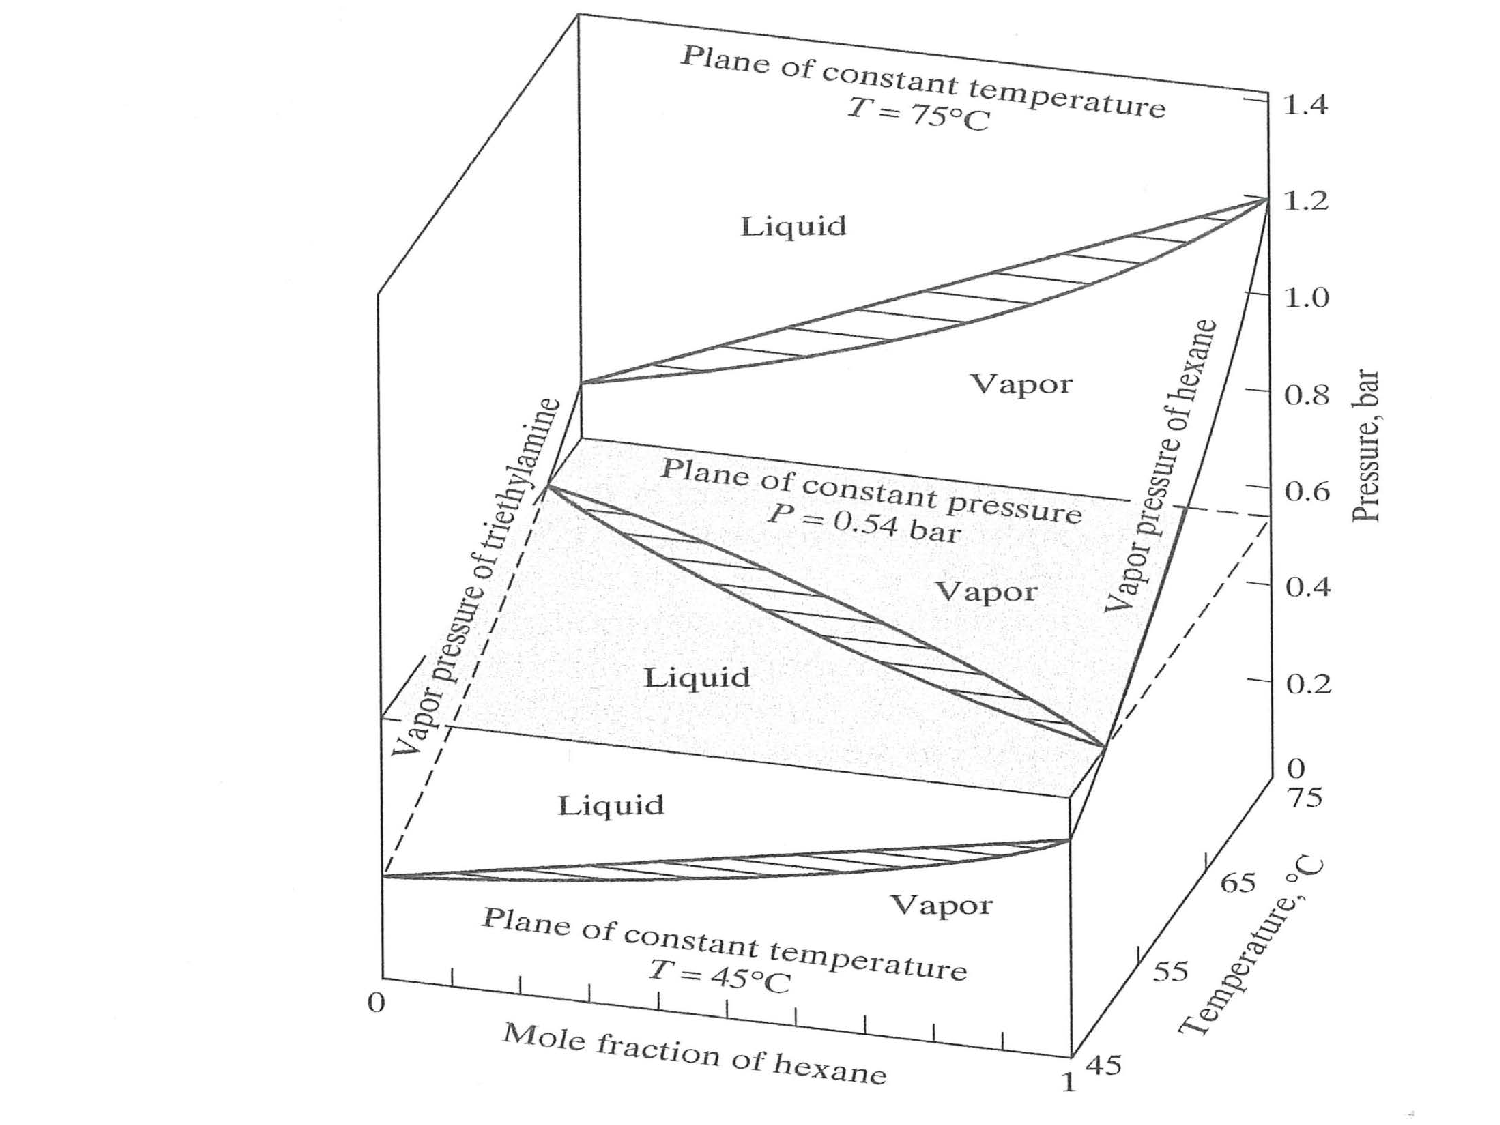
\includegraphics[width=9.cm,clip]{./../Pics/PTxy_diagram}}
       \begin{center}
            \tiny{{\bf Fig.} Hexane and triethylamine mixture (extracted from Sandler).}
            \end{center}
     \end{column} 
  \end{columns}
\end{frame}
\normalsize

%%%
%%% Slide
%%%
%\scriptsize
\begin{frame}
  \frametitle{$P$-$T$-$xy$ Diagram}
     \begin{center}
       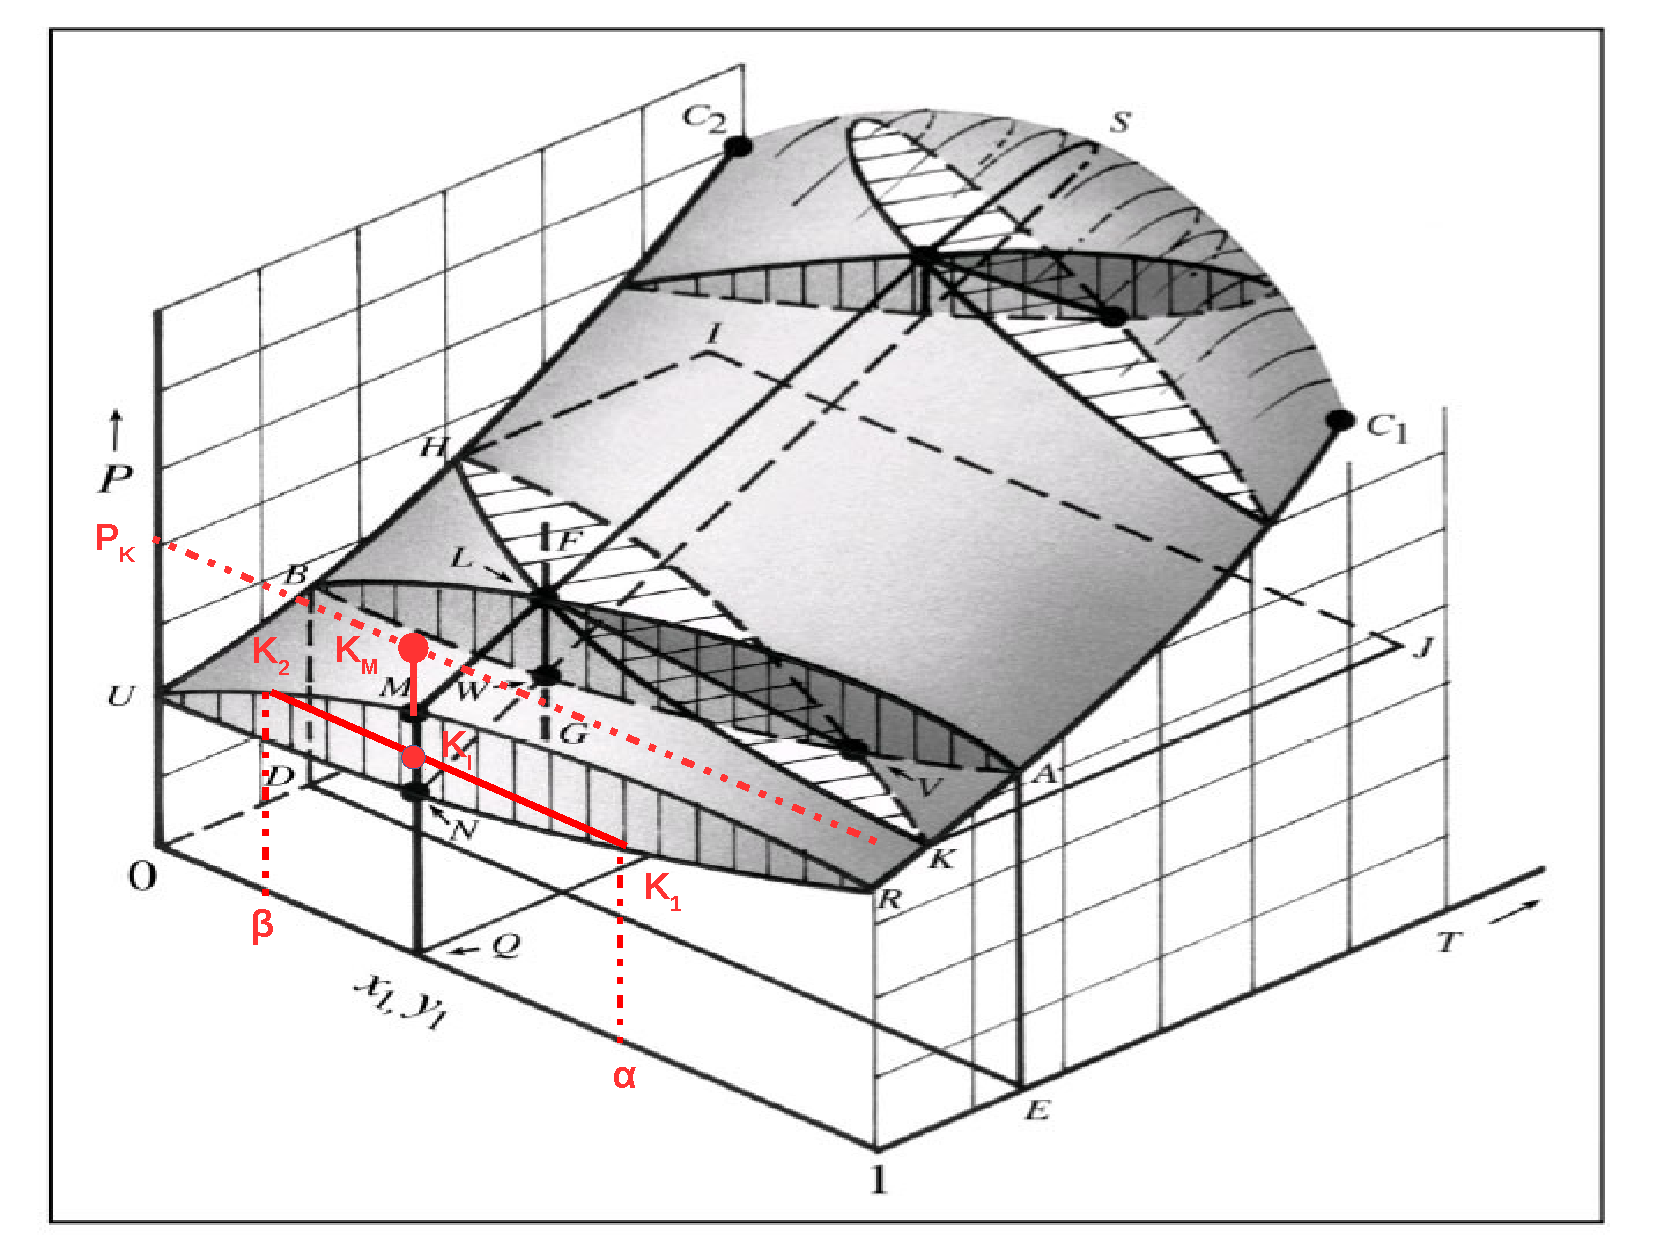
\includegraphics[width=.75\columnwidth,clip]{./../Pics/PTxy_Digram} %{./../Pics/PTxy_diagram2}
     \end{center}
\end{frame}
\normalsize


%%%
%%% Slide
%%%
\scriptsize
\begin{frame}
  \frametitle{$Pxy$ Diagrams} 
  \vspace{-0.8cm}
  \begin{columns}
     \begin{column}[l]{0.5\linewidth}
        \visible<1->{\hbox{\hspace{-1.7cm}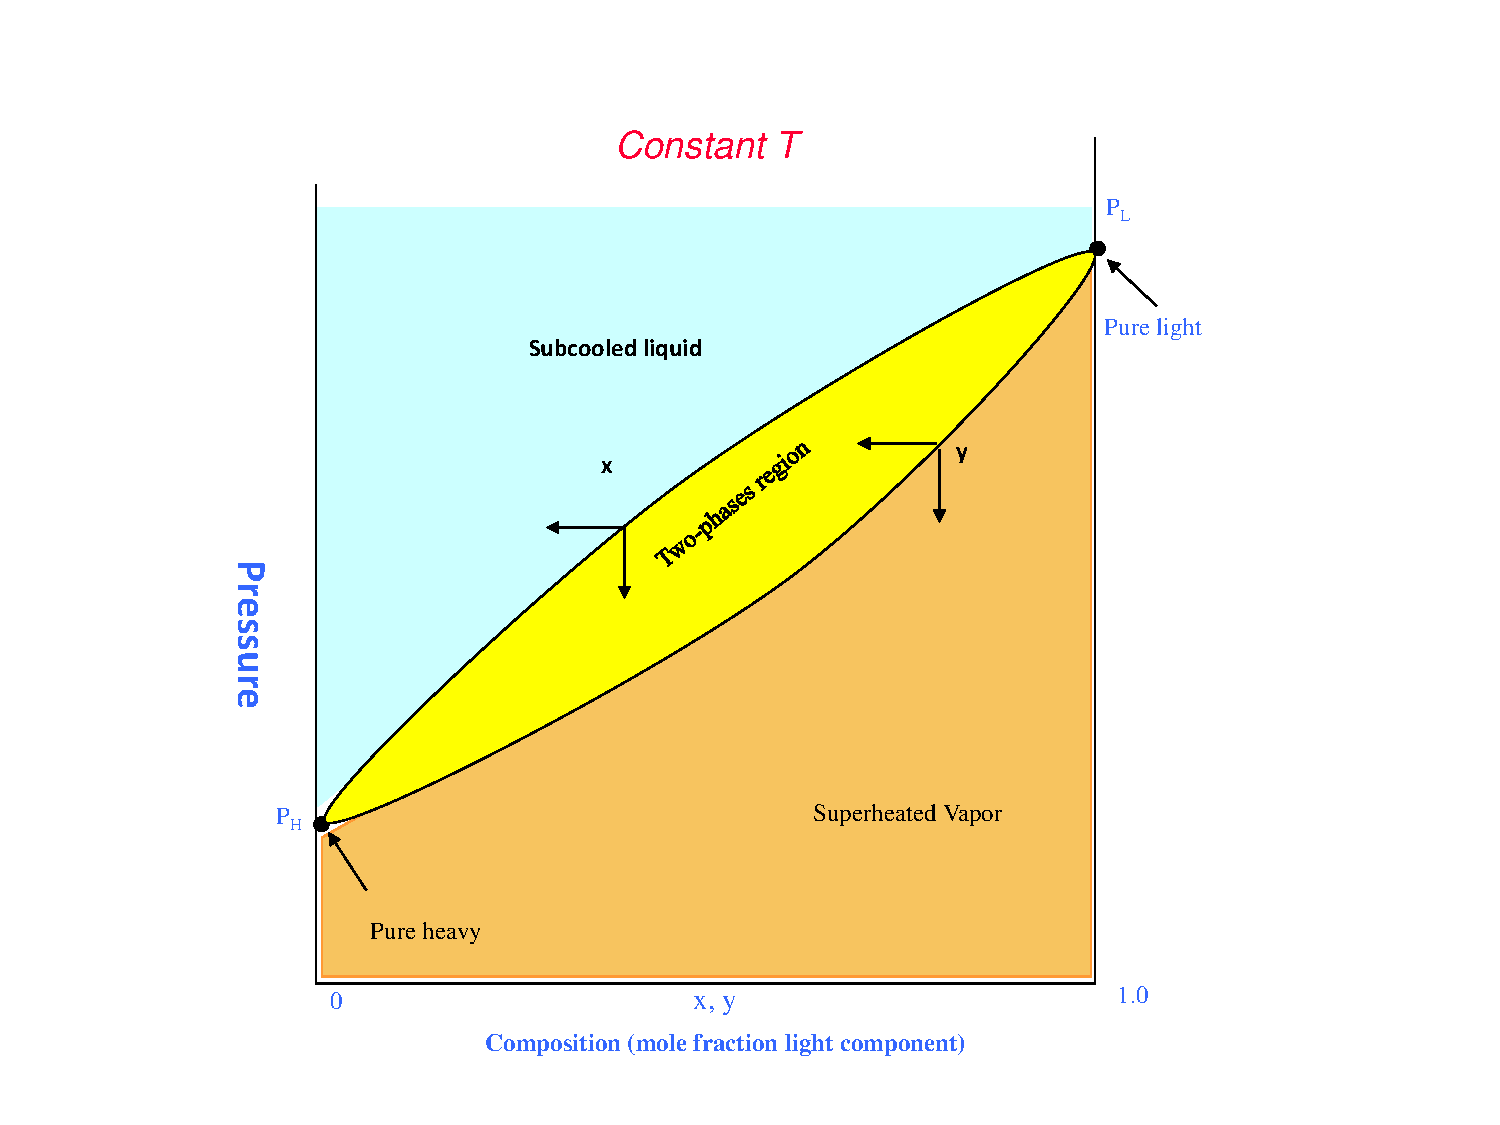
\includegraphics[width=1.6\linewidth,clip]{./../Pics/VLE_Pxy_Diagram1}}}
        %Upper curve: liquid phase composition $x$;\\
        %Lower curve: vapour phase composition $y$;
     \end{column}
     \begin{column}[l]{0.5\linewidth}
       \visible<2->{\hbox{\hspace{-1.7cm}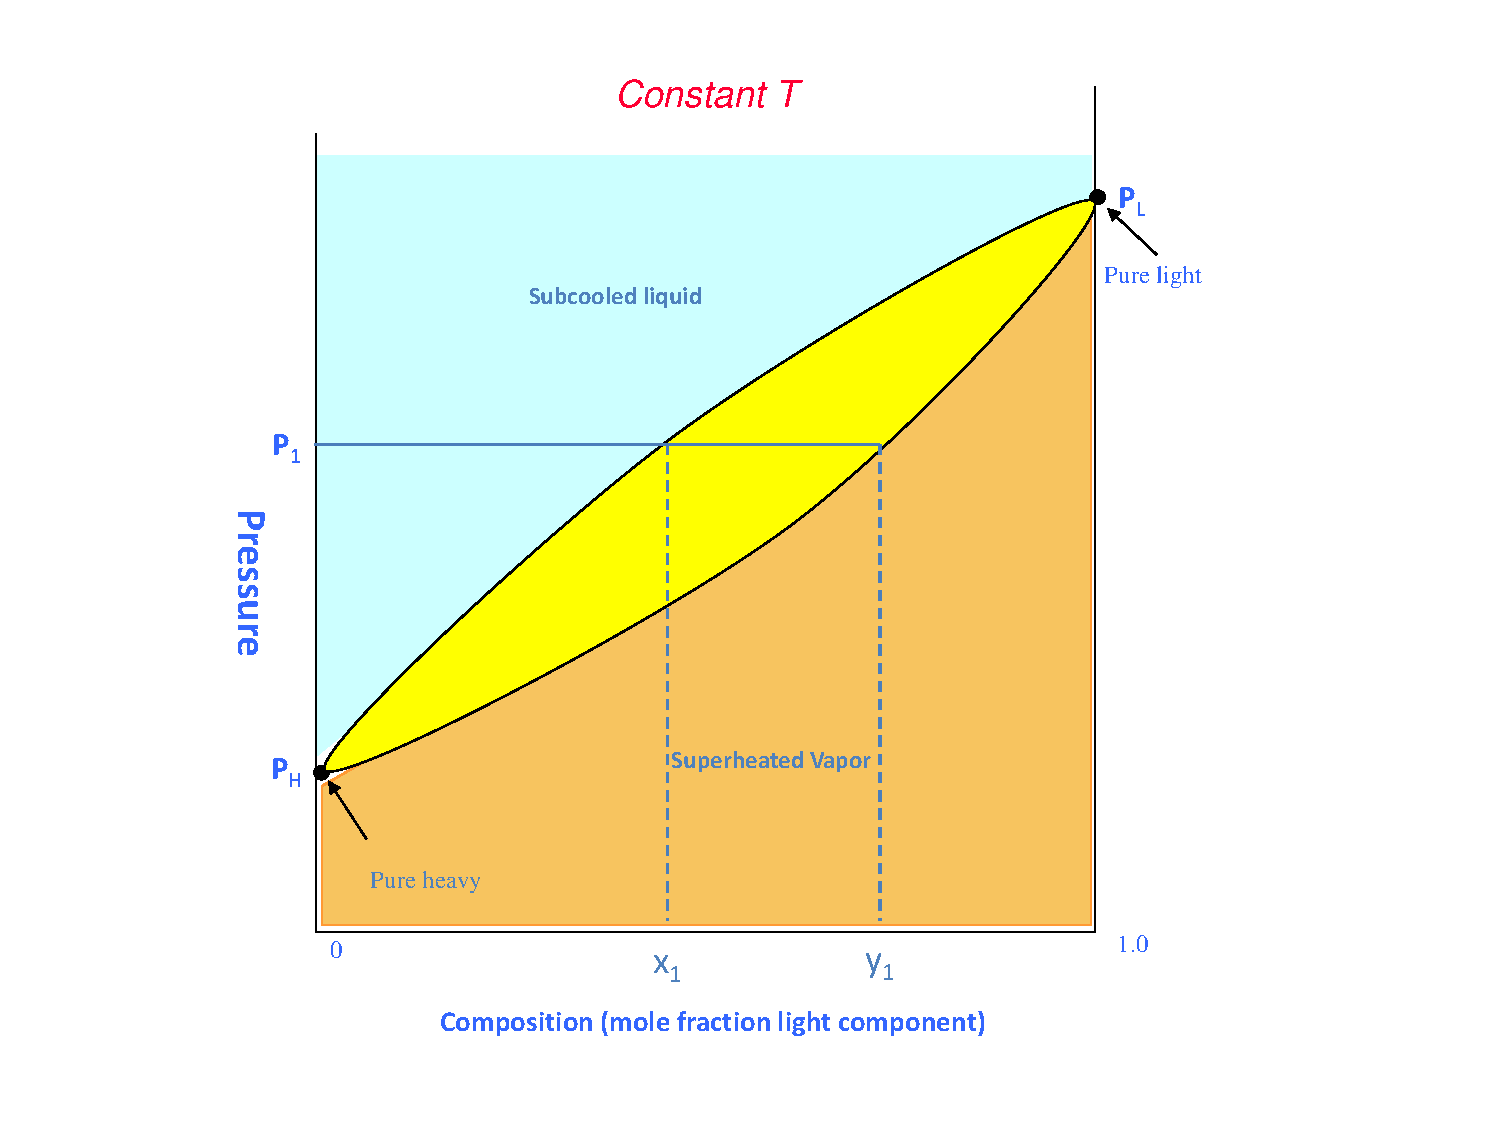
\includegraphics[width=1.6\linewidth,clip]{./../Pics/VLE_Pxy_Diagram2}}}
     \end{column}
  \end{columns}
         \visible<1->{Upper and lower curves represent liquid \red{($x$)} and vapour \red{($y$)} phases compositions, respectively.}\\
         \visible<2->{$P_{H}$ and $P_{L}$ are the vapour pressure of pure heavy and light components at $T$.}
\end{frame}
\normalsize


%%%
%%% Slide
%%%
%\scriptsize
\begin{frame}
  \frametitle{$Pxy$ Diagrams}
  \begin{columns}
     \begin{column}[l]{0.5\linewidth}
       \begin{enumerate}[i)]
          \item<1-> Consider a binary gaseous mixture with initial composition \red{$\left[x_{1}=0; y_{1}=y_{z}\right]$} and \blue{$\left[x_{2}=0; y_{2}=1-y_{1}\right]$} at $T$ and $P_{z}$;
          \item<2-> When $P$ is raised from $P_{z}$ to $P_{\text{DP}}$ (coordinate \red{R}), the mixture start condensating and the \blue{first droplet} of liquid is formed. \blue{$P_{\text{DB}}$} is called {\bf \red{\underline{dew point}}};
          \item<3-> Mixture composition at \red{R} is \red{$\left[x_{1}=x_{\text{DP}}; y_{1}=y_{z}\right]$} and \blue{$\left[x_{2}=1-x_{1}; y_{2}=1-y_{1}\right]$};
          \item<4-> As the pressure is further increased, more liquid is formed;
       \end{enumerate}
     \end{column}
     \begin{column}[l]{0.5\linewidth} 
        \visible<1->{\hbox{\hspace{-.0cm}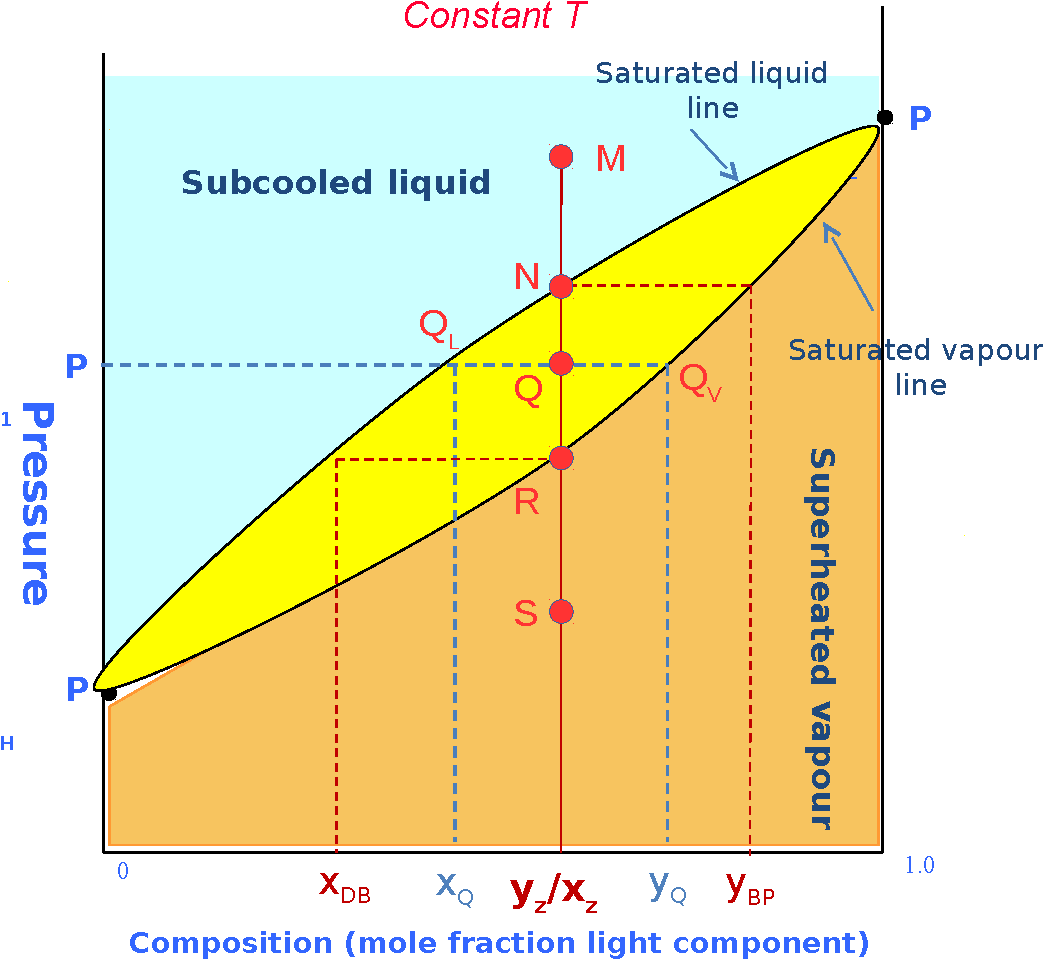
\includegraphics[width=1.\linewidth,clip]{./../Pics/VLE_Pxy_Diagram3b}}}
     \end{column}
  \end{columns}
\end{frame}
\normalsize

%%%
%%% Slide
%%%
%\scriptsize
\begin{frame}
  \frametitle{$Pxy$ Diagrams}
  \begin{columns}
     \begin{column}[l]{0.5\linewidth}
       \begin{enumerate}[i)]\setcounter{enumi}{3}
          \item<1-> At \red{Q} $\left(P_{1}\right)$, liquid and vapour are in equilibrium with composition \red{$\left[x_{1}=x_{\text{Q}}; y_{1}=y_{\text{Q}}\right]$} and \blue{$\left[x_{2}=1-x_{1}; y_{2}=1-y_{1}\right]$};
          \item<2-> Line linking $Q_{L}$ and $Q_{V}$ through $Q$ is called {\bf \red{\underline{tie line}}};
          \item<3-> When the pressure finally reaches \red{N}, the last bubble of vapour condensates and vanishes. \blue{$\left(P_{\text{BP}}\right)$} is called {\bf \red{\underline{bubble point}}} with composition \red{$\left[x_{1}=x_{\text{z}}; y_{1}=y_{\text{BP}}\right]$} and \blue{$\left[x_{2}=1-x_{1}; y_{2}=1-y_{1}\right]$};
          \item<4-> At \red{M}, the misxture is at \underline{subcooled liquid} state (\ie there is no longer vapour in the system) and the composition is \red{$\left[x_{1}=x_{\text{z}}; y_{1}=0\right]$} and \blue{$\left[x_{2}=1-x_{1}; y_{2}=0\right]$}.
       \end{enumerate}
     \end{column}
     \begin{column}[l]{0.5\linewidth} 
        \visible<1->{\hbox{\hspace{-.0cm}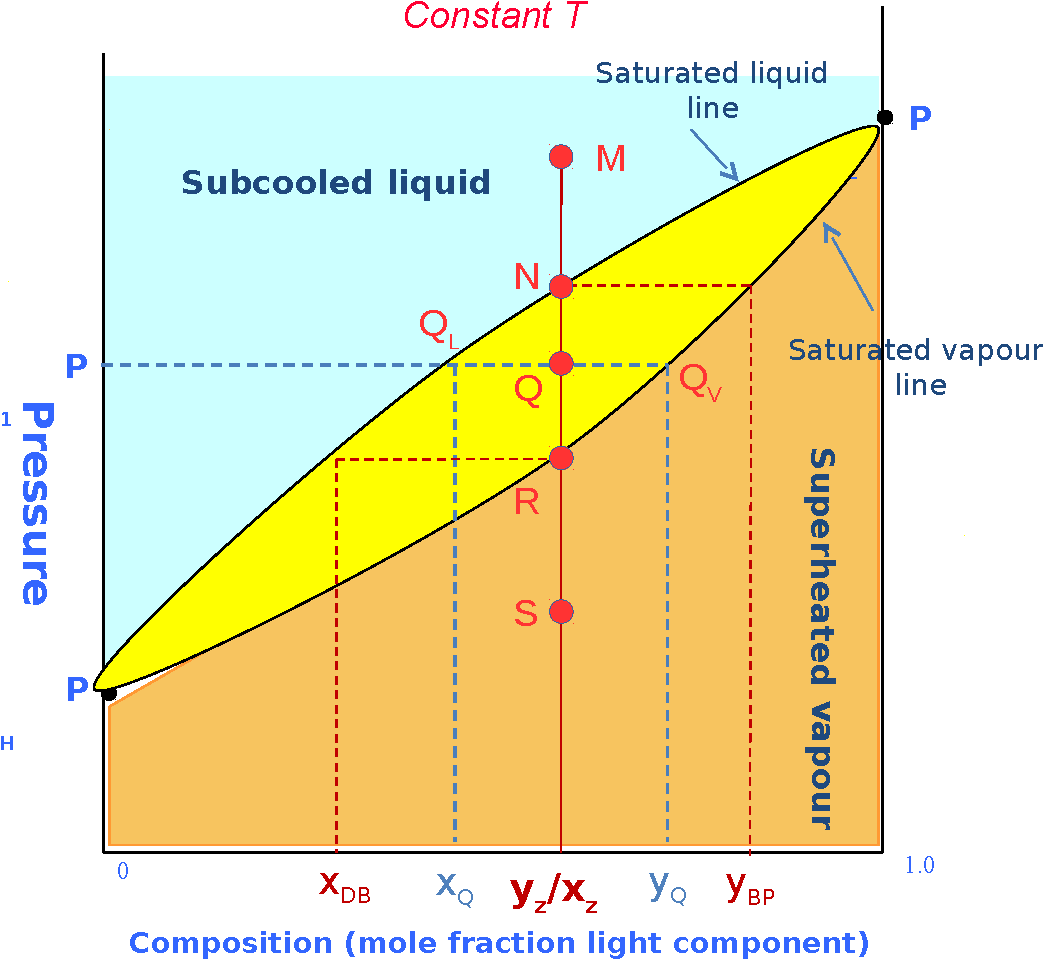
\includegraphics[width=1.\linewidth,clip]{./../Pics/VLE_Pxy_Diagram3b}}}
     \end{column}
  \end{columns}
\end{frame}
\normalsize


%%%
%%% Slide
%%%
%\scriptsize
\begin{frame}
  \frametitle{$xy$ Diagrams}
  \begin{columns}
     \begin{column}[l]{0.4\linewidth}
       \begin{enumerate}[i)]
          \item<1-> The $xy$ diagram for a binary system correlates the compositions of the liquid and vapour phases in equilibrium;
          \item<1-> They are designed assuming either constant $P$ or $T$ $\Longrightarrow$ though most industrial applications are isobaric.
       \end{enumerate}
     \end{column}
     \begin{column}[l]{0.6\linewidth}
        \visible<1->{\hbox{\hspace{-.0cm}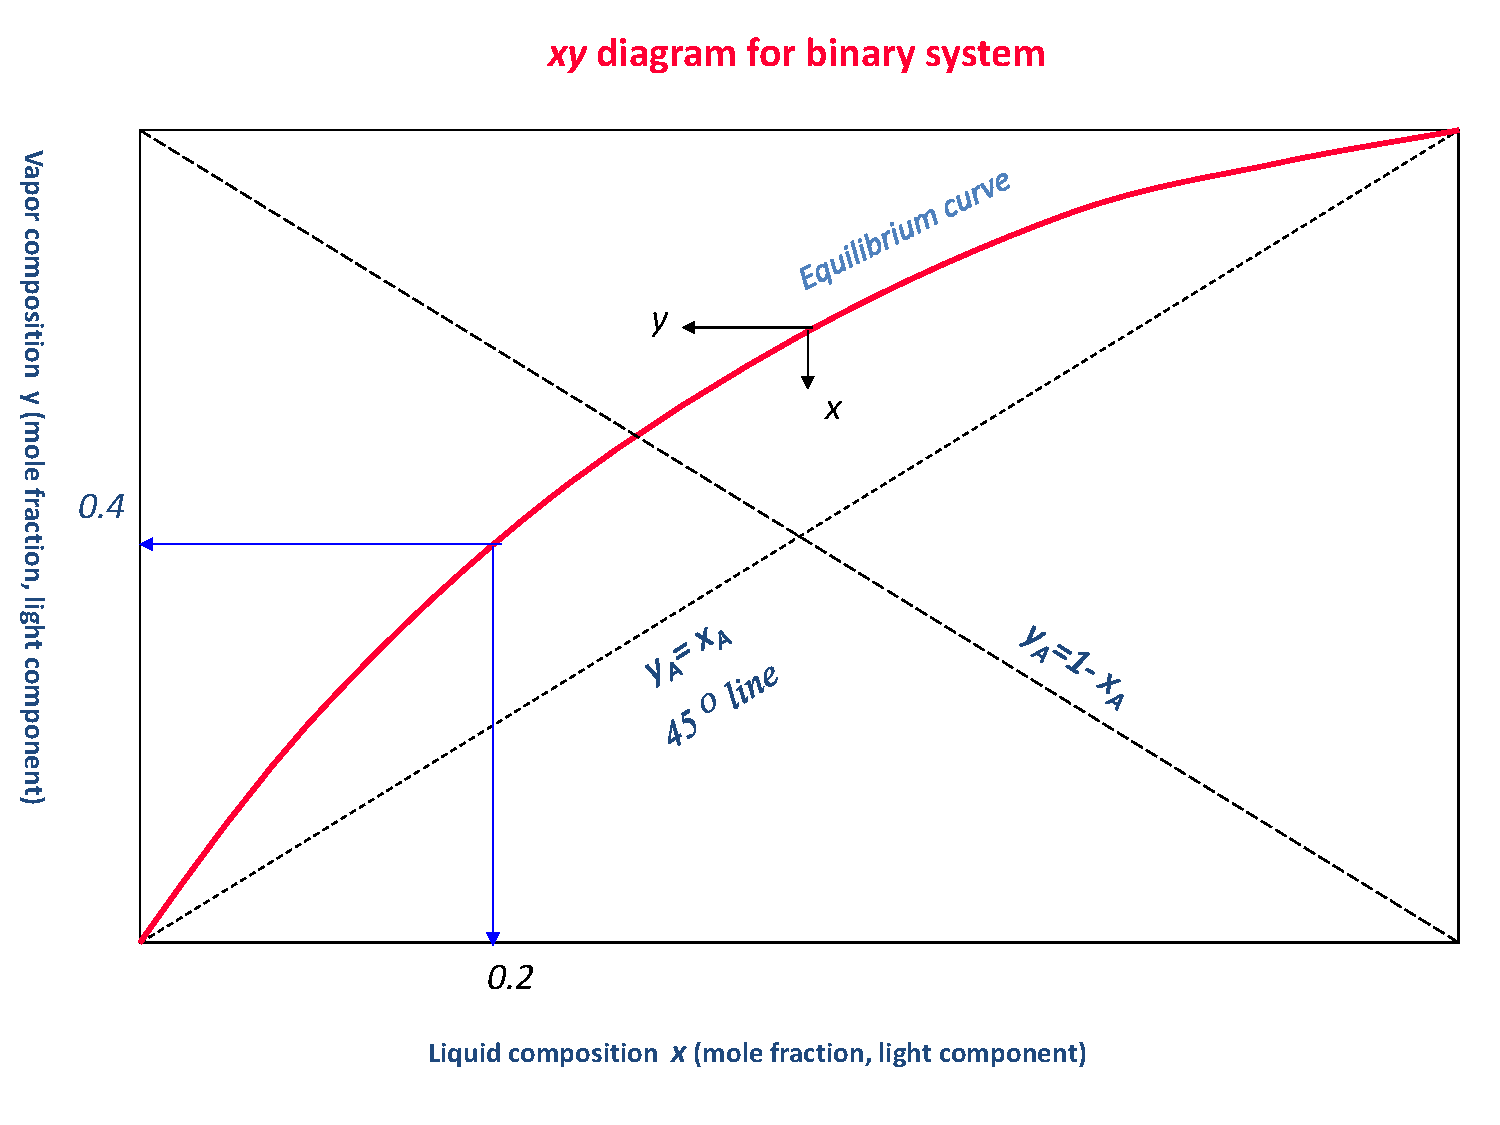
\includegraphics[width=1.\linewidth,clip]{./../Pics/VLE_xy_Diagram1}}}
     \end{column}
  \end{columns}
\end{frame}
\normalsize


%%%
%%% Slide
%%%
%\scriptsize
\begin{frame}
  \frametitle{$xy$ Diagrams: Ideal and Non-Ideal Solutions}
  \vbox{
     \hbox{\visible<1->{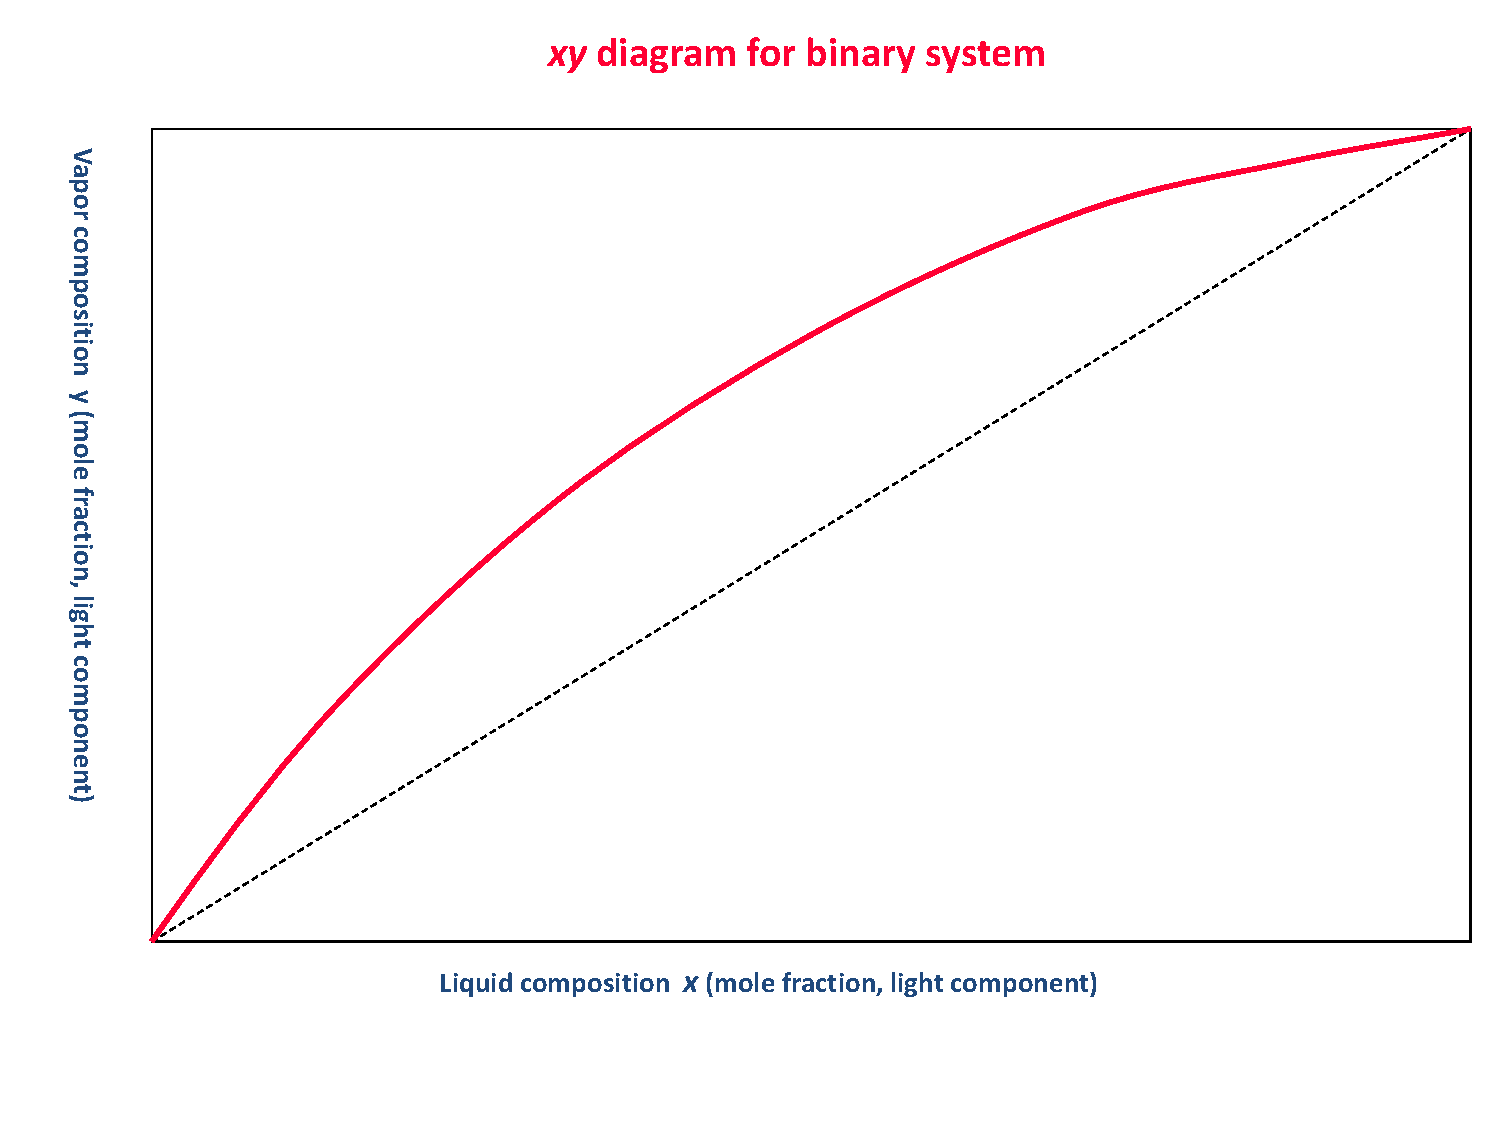
\includegraphics[width=5.5cm,height=4.cm,clip]{./../Pics/VLE_xy_DiagramIdeal}} \hspace{1cm}
           \visible<2->{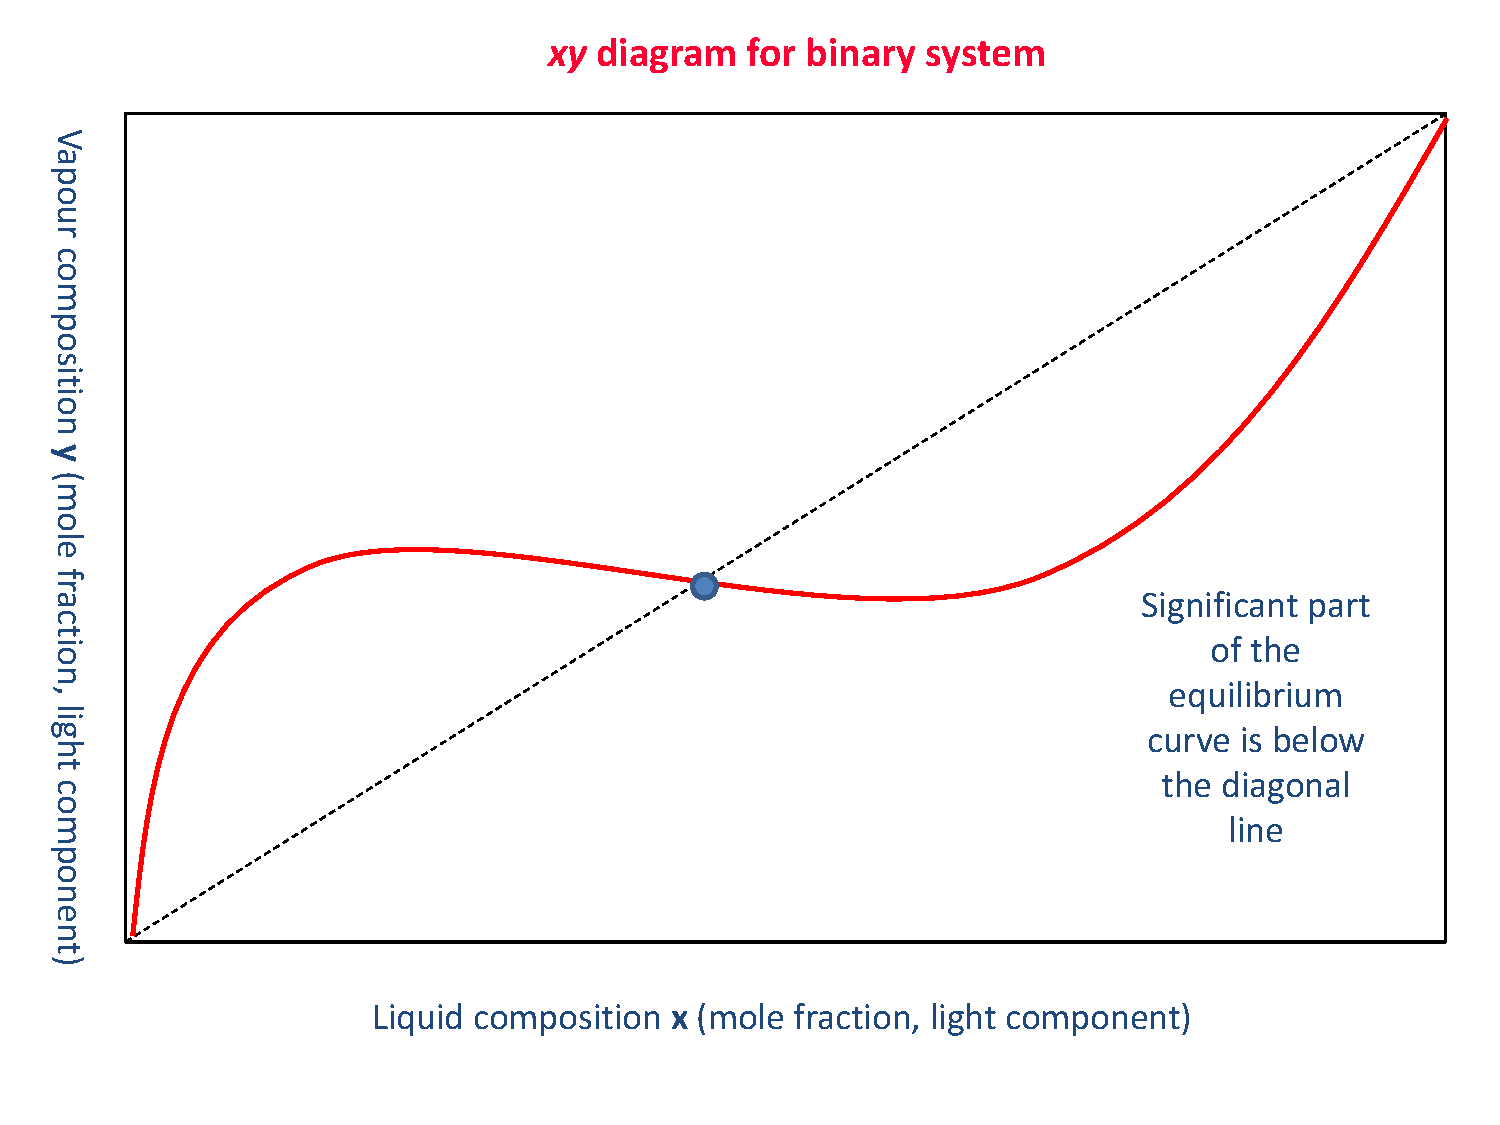
\includegraphics[width=5.5cm,height=4.cm,clip]{./../Pics/VLE_xy_DiagramNonIdeal1}}}
  \vspace{-0.2cm}
  \hbox{\hspace{4cm}
        \visible<3->{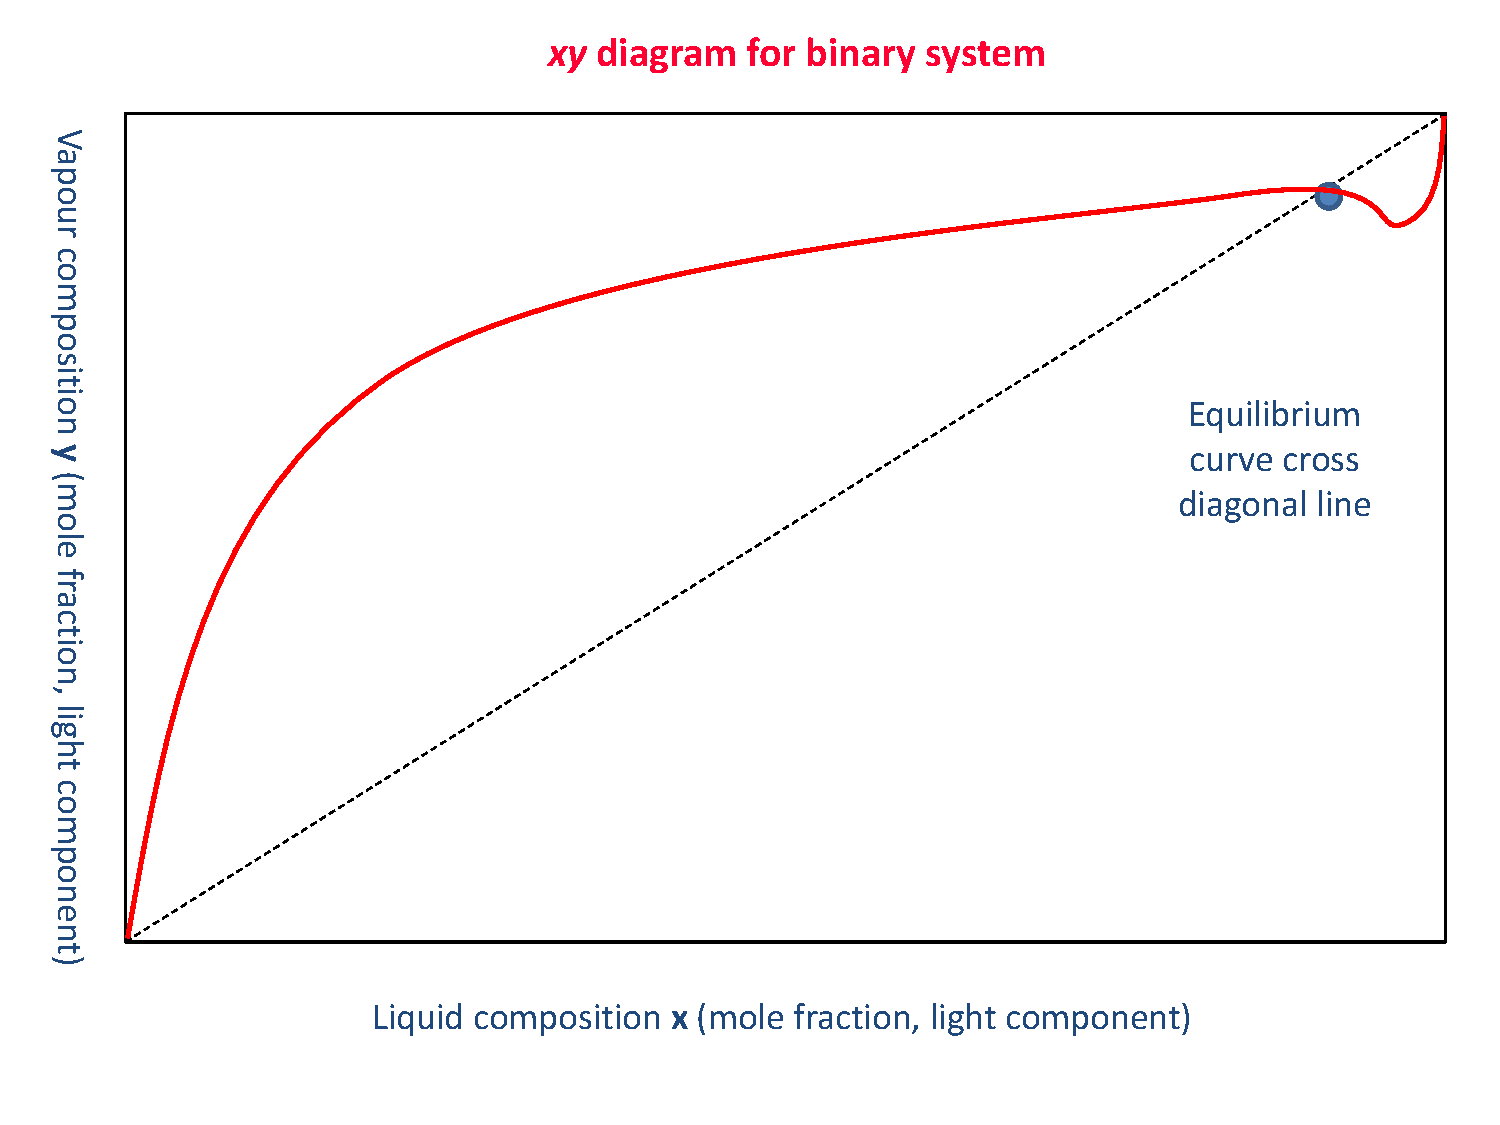
\includegraphics[width=5.5cm,height=4.cm,clip]{./../Pics/VLE_xy_DiagramNonIdeal2}}}
  }
\end{frame}
\normalsize


%%%
%%% SUBSECTION
%%%
\subsection{Simple Models}

%%%
%%% Slide
%%%
\begin{frame}
  \frametitle{General Remarks}
  \begin{enumerate}[i)]
      \item<1-> \blue{VLE models} aim for mathematical descriptions of the PVT behaviour of mixtures at equilibrium conditions:
         \begin{enumerate}[a)]
            \item<1-> Prediction of \blue{vapour and liquid compositions} at given $T$ and $P$;
            \item<1-> \underline{Basis for process modelling}.
         \end{enumerate}
      \item<2-> Two simple models:
         \begin{enumerate}[a)]
            \item<2-> \textcolor{blue}{Raoult's law};
            \item<2-> \textcolor{blue}{Henry's law}.
         \end{enumerate}
  \end{enumerate}
\end{frame}

%%%
%%% Slide
%%%
\begin{frame}
  \frametitle{Raoult's Law}
  \begin{enumerate}[i)]
      \item<1-> Main assumptions:
         \begin{enumerate}[a)]
             \item<1-> \textcolor{blue}{vapour phase} behaves as an {\bf ideal gas} $\Longrightarrow$ low to moderate pressures;
             \item<1-> \textcolor{blue}{liquid phase} is an {\bf ideal solution}.
         \end{enumerate}
         \visible<2->{\begin{block}{\begin{center}\normalsize{Raoult's Law}\end{center}}
              \begin{displaymath}
                  \blue{ P_{i}= y_{i}P = x_{i} P_{i}^{\text{sat}}\left(T\right),} \hspace{2cm} \blue{\forall i\in\left\{1,2,\cdots,\mathcal{C}\right\}}
              \end{displaymath}
         \end{block}
         where $P_{i}=y_{i}P$ is the {\bf partial pressure} of species {\it i} in the vapour phase.}
      \item<2-> This equation indicates that the partial pressure of a component in an ideal solution is equal to the product of the species mole fraction and its vapour pressure (of the pure component);
      \item<3-> Two major constraints:
         \begin{enumerate}
             \item<2-> Mass balance of both phases: $\sum\limits_{i=1}^{\mathcal{C}} x_{i} = 1$ and $\sum\limits_{i=1}^{\mathcal{C}} y_{i} = 1$
             \item<2-> {\bf Ideal solution:} \textcolor{blue}{$x_{i}\rightarrow 1$}. Also species {\bf must} be chemically similar (i.e., size, same chemical nature, e.g., isomers such as ortho-, meta-, and para-xylene) 
         \end{enumerate}
  \end{enumerate}
\end{frame}


%%%
%%% Slide
%%%
\begin{frame}
  \frametitle{Raoult's Law: Ideal gas mixture properties}
  \begin{enumerate}
      \item<1-> Dalton's Law: \textcolor{blue}{$P=\sum\limits_{i=1}^{\mathcal{C}}P_{i}=\sum\limits_{i=1}^{\mathcal{C}}y_{i}P$}
      \item<2-> Amagat's Law: \textcolor{blue}{$V^{t}=\sum\limits_{i=1}^{\mathcal{C}}V_{i}^{t} = \sum\limits_{i=1}^{\mathcal{C}} y_{i}V^{t}$}
      \item<3-> Kay's rule: pseudo-critical pressure \textcolor{blue}{$\left(P_{c}^{t}=\sum\limits_{i=1}^{\mathcal{C}}y_{i}P_{c,i}\right)$} and temperature \textcolor{blue}{$\left(T_{c}^{t}=\sum\limits_{i=1}^{\mathcal{C}}y_{i}T_{c,i}\right)$}. 
  \end{enumerate}
\end{frame}

%%%
%%% Slide
%%%
\begin{frame}
  \frametitle{Raoult's Law: Dew and Bubble Point Calculations}
         \visible<1->{\begin{block}{\begin{center}\normalsize{Dew Point Calculation}\end{center}}
                         \begin{enumerate}[i)]
                            \item Given $y_{i}$ and $T$, calculate \blue{$x_{i}$} and \blue{$P$}
                            \item Given $y_{i}$ and $P$, calculate \blue{$x_{i}$} and \blue{$T$}
                         \end{enumerate}
                      \end{block}}
         
         \visible<2->{\begin{block}{\begin{center}\normalsize{Bubble Point Calculation}\end{center}}
                         \begin{enumerate}[i)]
                            \item Given $x_{i}$ and $T$, calculate \blue{$y_{i}$} and \blue{$P$}
                            \item Given $x_{i}$ and $P$, calculate \blue{$y_{i}$} and \blue{$T$}
                         \end{enumerate}
                      \end{block}}
\end{frame}

%%%
%%% Slide
%%%
\begin{frame}
  \frametitle{Generalised Relation for VLE in Ideal Mixtures}
  \begin{enumerate}[i)]
      \item<1-> Raoult's law is a particular case of a more general relation involving \textcolor{blue}{vapour-liquid mixtures} (that we will see with more details on Module 4),
           \visible<2->{\begin{displaymath}
              f_{i}^{\left(L\right)}\left(T,P,\underline{x}\right) = f_{i}^{\left(V\right)}\left(T,P,\underline{y}\right)
           \end{displaymath}
           where $\underline{x}$ and $\underline{y}$ represent the array of compositions in the liquid and vapour phases, respectively, and \blue{$f$} is the fugacity of the fluid;}
      \item<3-> For low-pressure VLE,
           \visible<3->{\begin{displaymath}
               \textcolor{blue}{y_{i}P=x_{i}\gamma_{i}P_{i}^{\text{sat}}}
           \end{displaymath}}
      \item<4-> The activity  coefficient of species $i$, \red{$\gamma_{i}$}, is a thermodynamic property that indicates \blue{$\lq$how much a solution will deviate from the ideal solution behaviour'};
      \item<4-> For an ideal solution, $\gamma_{i}=1$, and the equation above becomes the Raoult's law.  
  \end{enumerate}
\end{frame}

%%%
%%% Slide
%%%
\begin{frame}
  \frametitle{Henry's Law}
  \begin{enumerate}[i)]
      \item<1-> Raoult's law requires vapour pressure data $\left(\text{\ie} P_{i}^{\text{sat}}\right)$, thus:
        \begin{enumerate}[a)]
            \item<1-> It is not applicable if $T\geq T_{c,i}$;
            \item<1-> Does not take into account gasses dissolved in the liquid.
        \end{enumerate}
      \item<2-> \red{Henry's law} was developed to model the concentration of gases dissolved in liquids (\ie gases solubility in liquid solutions). It can only be used for \underline{very small concentrations of gaseous species in solutions}, 
         \visible<2->{\begin{block}{\begin{center}\normalsize{Henry's Law}\end{center}}
                         \begin{displaymath}
                            \blue{y_{i}P = x_{i}\mathcal{H}_{i},} \hspace{2cm} \blue{\forall i\in\left\{1,2,\cdots,\mathcal{C}\right\}}
                         \end{displaymath}
                      \end{block}}
  \end{enumerate}
  \visible<2->{
 \begin{table}
  \begin{center}
    \begin{tabular}{l r || l r }
      \hline
       {\bf Gas}    &  ${\bf \mathcal{H}\text{ (bar)}}$ & {\bf Gas}    &  ${\bf \mathcal{H}\text{ (bar)}}$ \\
      \hline
         Acetylene  &   1350                            & He           &  126600 \\
         Air        &   72950                           & H$_{2}$      &  71600  \\
         CO$_{2}$    & 1670                              & H$_{2}$S     & 550 \\
         CO         &  54600                            &  CH$_{4}$    &  41850 \\
         C$_{2}$H$_{6}$ & 30600                          &  N$_{2}$     & 87650  \\
         Ethylene  & 11550                              & O$_{2}$      & 44380 \\
      \hline
    \end{tabular}
    \caption{Henry's constant for gases dissolved in water at 25$^{\circ}$C.}
  \end{center}
\end{table}}
\end{frame}


%%%
%%% Slide
%%%
\begin{frame}
  \frametitle{K-Value Correlations}
  \begin{columns}
     \begin{column}[l]{0.5\linewidth}
        \begin{enumerate}[i)]
           \item<1-> Equilibrium ratio, $K_{i}$
               \visible<1->{\begin{displaymath}
                  K_{i} = \frc{y_{i}}{x_{i}}
               \end{displaymath}}
           \item<2-> With Raoult's law:
               \visible<2->{\begin{displaymath}
                  K_{i} = \frc{P_{i}^{\text{sat}}}{P}
               \end{displaymath}}
           \item<3-> With modified Raoult's law:
               \visible<3->{\begin{displaymath}
                  K_{i} = \frc{\gamma_{i}P_{i}^{\text{sat}}}{P}
               \end{displaymath}}
        \end{enumerate}
     \end{column}
     \begin{column}[l]{0.5\linewidth}
        \begin{center}
          \hspace{-.8cm}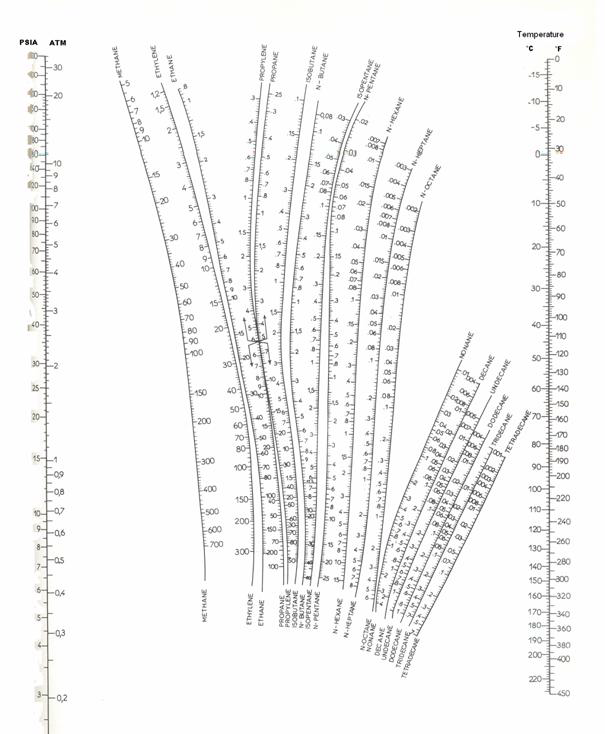
\includegraphics[width=5.7cm,clip]{./../Pics/02_07_fig_02.png}
          
          \tiny{\bf{Fig.:} DePriester chart for several hydrocarbons (extracted from Smith {\it et al.}).}
        \end{center}
     \end{column}
   \end{columns}
\end{frame}

%%%
%%%  SECTION
%%%
\subsection{Industrial Applications for VLE of Mixtures: Flash Calculation}

%%%
%%% Slide
%%%
\begin{frame}
  \frametitle{Flash Calculation}
  \begin{columns}
     \begin{column}[c]{0.5\linewidth}
       \visible<3->{\hspace{-1cm}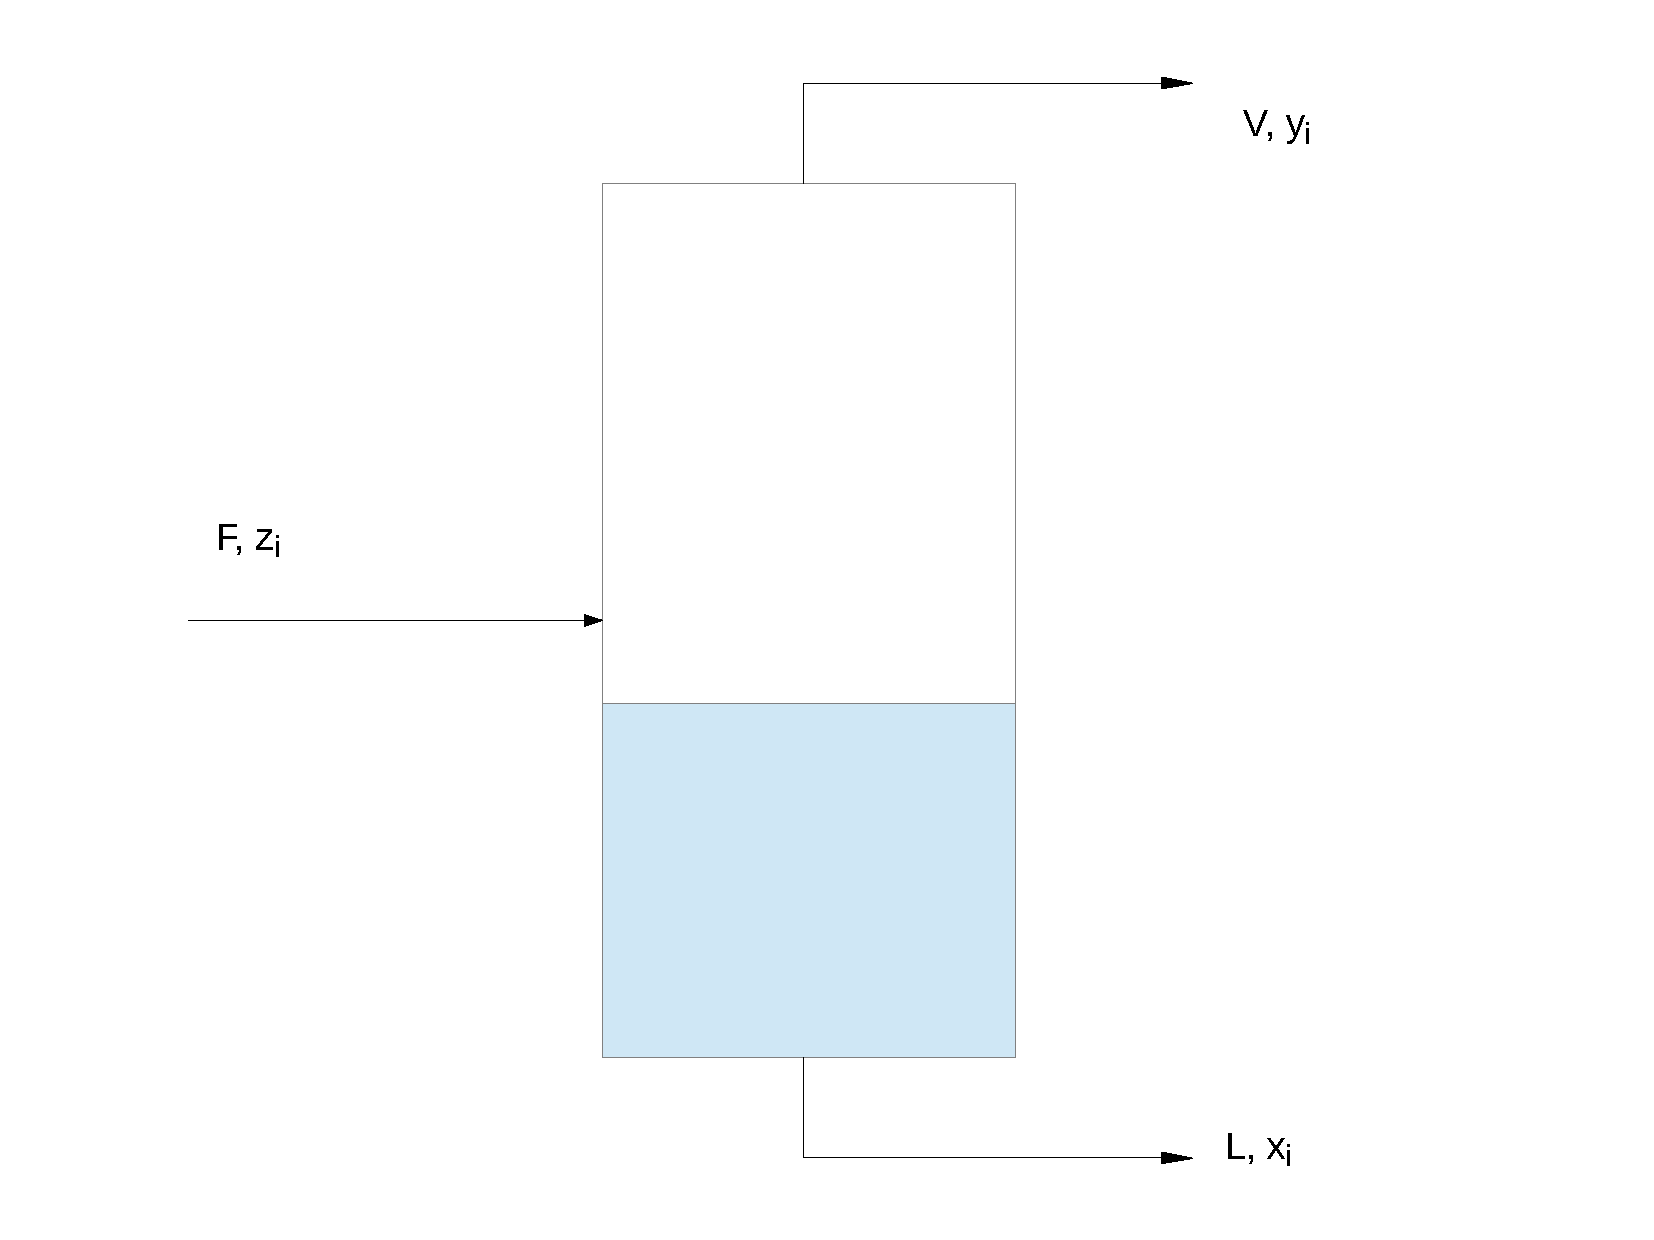
\includegraphics[width=1.3\linewidth,clip]{./../Pics/Flash_VLE}}
     \end{column}
     \begin{column}[l]{0.5\linewidth}
        \begin{enumerate}[i)]
           \item<1-> If a fluid mixture is at liquid state with pressure larger than the associated bubble point pressure; % $\left(\text{i.e., }P \leq P_{\text{BP}}\right)$;
           \item<2-> Part of the fluid evaporates \textcolor{blue}{(or {\it flashes})} when the pressure is reduced leading to a two-phase system -- vapour and liquid in equilibrium;
            \item<3-> This phenomenon is often called \textcolor{blue}{\it flash} and is the most important application of VLE;
            \item<4-> Thus, a feeding stream $F$ with overall composition $z_{i}$ is separated into vapour ($V$) and liquid ($L$) streams with compositions $y_{i}$ and $x_{i}$, respectively. 
        \end{enumerate}
     \end{column}
   \end{columns}
\end{frame}

%%%
%%% Slide
%%%
\begin{frame}
  \frametitle{Flash Calculation}
     
         \visible<1->{\begin{block}{\begin{center}\normalsize{Overall Mass Balance}\end{center}}
                         \begin{displaymath}
                            F = V + L = 1,
                         \end{displaymath}
                         where $F$, $V$ and $L$ are molar fractions of the streams.
                      \end{block}}

         \visible<2->{\begin{block}{\begin{center}\normalsize{Material Balance for Component \blue{$i$}}\end{center}}
                         \begin{displaymath}
                            F z_{i} = x_{i}L + y_{i}V \hspace{1.cm}\text{ with }\hspace{1cm} K_{i}=\frc{y_{i}}{x_{i}},
                         \end{displaymath}
                         where \blue{$z_{i}$} is the molar composition of the feeding stream ($F$). This leads to the composition of species \blue{$i$} in the \red{vapour phase at equilibrium,}
                         \begin{displaymath}
                            y_{i} = \frc{z_{i}K_{i}}{1 + V\left(K_{i}-1\right)}.
                         \end{displaymath}
                      \end{block}}
  
\end{frame}
%%%
%%% Slide
%%%
\begin{frame}
  \frametitle{Flash Calculation}
     
        \visible<1->{\begin{block}{\begin{center}\normalsize{Flash Calculation}\end{center}}
                         As $\summation[y_{i}]{i=1}{\mathcal{C}}=1$,
                         \begin{displaymath}
                            \blue{\summation[\frc{z_{i}K_{i}}{1+V\left(K_{i}-1\right)}]{i=1}{\mathcal{C}} = 1.}
                         \end{displaymath}
                         \red{Solving a $P-T$ flash problem is to \underline{find V that satisfies this equation.}}
                      \end{block}}
  
\end{frame}


\section{Summary}

%%%
%%% Slide
%%%
%\scriptsize
\begin{frame}
 \frametitle{Summary}
   \begin{enumerate}[(i)]
     \item Stability conditions/criteria;
     \item Qualitative analysis of VLE -- efficient use of graphical representation of $P$, $T$ and composition of species;
     \item Introduction to generalised relation for VLE in non-ideal mixtures;
     \item Raoult and Henry's laws; 
     \item Industrial application for VLE: Flash problem.
   \end{enumerate}
\end{frame}


\end{document}
 
